
\chapter{Experimental Observations in SW06}
\section{Shallow water '06 experiment}
The multi-institutional SW06 experiment was conducted on the New
Jersey continental shelf (Fig. \ref{fig:sw06site} ) from July to
September 2006 at a location where internal wave activity has been
observed and studied in the past\cite{jasa4,Tang1} . To assess the combined acoustic and oceanographic relationship between the acoustic wave propagation and the internal waves, the geometry of the receiving arrays and the environmental sensors were placed in a region shown in Fig\ref{fig:mooring}. R/V Oceanous took continuous measurements of several internal waves during ?? to ?? from formation to growing, propagation, and finally the decay of the IW. \ref{7} See Fig ??. The dominant direction of these waves that are tidally generated on the continental shelf break, is estimated based on 60 IW events and is shown in Fig.?? The direction of most of these waves is between $300^o-330^o$ with respect to the north ($0^o$) and the propagation path as well as the decay rate varies considerably from one wave to another. Here we
focus on a particular internal wave event on August 17, 2006, for
which a complete set of acoustic and environmental data were
collected simultaneously. In addition, ISW surface signatures were
captured continuously by the on-board radars of two research vessels
prior to the arrival of, and during the passing of, the ISW packet
over the acoustic track. The acoustic wave field variation is
studied during this process.


During SW06, several acoustic sources were used to transmit sound while environmental data were collected
simultaneously\cite{WHOI}. Here we discuss the acoustic data from a
particular acoustic source (NRL 300Hz) on the mooring denoted SW45
(see Fig. 1). The source was located 72 m below the sea surface and
10.5 m above the sea floor at $39^{o}10.957'$ N, $72^o56.575'$ W,
and transmitted 2.0489 second Linear Frequency Modulating (LFM)
signals from 270 to 330 Hz every 4 seconds. Transmissions continued
for 7.5 minutes and then repeated every half hour.  A vertical and
horizontal receiver array (the "Shark VHLA") on mooring SW54 was
located at $39^o01.252'$ N, $73^o02.983'$ W, about 20.2 km south of
the NRL source.  The vertical part of the receiver array consisted
of 16 hydrophones with 3.5 m spacing and was positioned in the water
column from 13.5 m to 77.75 m below the surface. The horizontal part
of the array consisted of 32 hydrophones on the seafloor with
spacing of 15 m, providing 478 m of horizontal aperture. The
sampling rate of the array was 9765.625 Hz. The acoustic track and
the locations of the source and receiver as well as the horizontal
and vertical array configurations are shown in Fig. 1. The water
depth along the acoustic track was about 80 m.


\subsection{Internal wave events in SW06}

Figure \ref{fig:temp} shows the temperature records at the acoustic
source mooring SW45, the midpoint SW20, and the receiver mooring
SW54 from 20:00 to 23:00 GMT on August 17, 2006. A solitary internal wave arrived at the receiver around 21:15 GMT, followed by a calm
period of about 20 minutes. At around 21:40 GMT, the leading front
of a strong ISW packet passed the receiver position. The ISW packet
caused a sudden increase in the thermocline depth. At 22:20 GMT, the
water temperature decreased slowly until 09:00 GMT the next day. The
leading wave front was observed at SW20 at 22:02 and at SW45 at
22:15 GMT, respectively. If we assume the leading wave front is
linear (it is not) and the wave speed is constant along the wave
front, this suggests an angle of about $5^o$ between the advancing
front and the acoustic track.

\section{Event 50/Rosey}
\subsection{Ship position and experiment setup}
On August 17, 2006, at about 18:00 GMT, the R/V Sharp from the
University of Delaware was located at $38^o59.262'$ N, $72^o57.492'$ W and
the R/V Oceanus from the Woods Hole Oceanographic Institution (WHOI)
was located at $38^o57.426'$ N, $72^o56.676'$ W. Both platforms observed
the origination of an ISW near the shelf break. This event was named
Event 50 on R/V Sharp and Rosey on R/V Oceanus.

Our goal is specifically to check the relationship between internal wave and acoustic wave propagation. In particular we seek to understand the acoustic wave propagation mechanisms governed by the direction of the acoustic track relation to the internal wave front. 



Fig.?? shows a schematic depicting different propagation mechanisms for an acoustic wave depending on its propagation track angle with the front of the internal wave. then mechanism changes form adiabatic to mode coupling, refraction depending on the angle[???]. In this work, we will explain theoretically and will also show this behavior from experimental observations. Based on this theory, an experiment was designed and conducted during summer 2006 [SW06]. The position of the source and receiver during this experiment is shown in Fig.\ref{fig:moorings}.


Figures 1(a) and 1(b) show the track of each vessel following this
event from 18:00 GMT on August 17 to 02:00 GMT on August 18, 2006.
The R/V Sharp's track was semi circular, centered at the WHOI
vertical and horizontal line array (Shark VHLA) with the ship being
positioned on the trough of the leading ISW front and moving with
the advancing front. The R/V Oceanus followed the same ISW packet
from its initial location, while keeping a watch on the advancing
wave front. Reversals in the track of R/V Oceanus indicate where the
wave packet was crossed, and during these periods, intensive
profiling of temperature, density, turbulence and sound velocity was
conducted.

The two ships observed different parts of the ISW front, thus
providing a large spatial coverage. The surface signatures of the
ISW were digitally recorded by on-board ship radar images every 30
seconds. Combined radar images from the two vessels, each about 11.1
km in diameter, covered the receiver and about two thirds of the
acoustic track. Mm. 1 shows a movie of the ships' radar images
following the ISW during this event, from 18:00 GMT on 17 August to
02:00 GMT on 18 August, 2006. In this paper we discuss two
situations: (1) when the ISW packet had not reached the acoustic
track [time period $T_{g1}$ (20:30 to 20:37 GMT)] and (2) when the ISW
occupied most of the acoustic track [time period $T_{g2}$ (22:00 to 22:07
GMT)]. The radar images from both vessels at 20:30 GMT and 22:00 GMT
are shown in Figs. 1(a) and 1(b) respectively.

At 20:30 GMT, the R/V Sharp radar showed 10 distinct ISW fronts in a
packet. At the same time, the R/V Oceanus radar showed 7 wave fronts
with less curvature. The spacing between wave fronts in the packet
varied from ~ 0.4 to 0.5 km for the leading wave fronts to ~ 0.2 to
0.3 km for the trailing waves. The ISW direction of propagation was
about compass direction $300^o$.

At 22:00 GMT, most of the acoustic track including the receiver
array was occupied by the ISW packet [see Fig. 1(b)]. The physical
characteristics of the ISW packet during this time were similar to
those at 20:30 GMT, except that its propagation direction was
slightly changed. The R/V Oceanus observed the ISW propagation
direction close to the receiver to be about 310o. At the middle of
the acoustic track (SW20), a propagation direction of 305o was
observed on RV Sharp. Note that the wave front was curved so there
is a natural discrepancy between the propagation directions observed
by the two ships. The angle between the ISW fronts and the acoustic
track at midpoint was approximately 5o and varied along the acoustic
track. The average speed of the ships following the ISW packet was
about 1.8 to 2.0 knots, which was similar to the ISW propagation
speed.
\subsection{Temperature measurement}
The SW45 mooring had eleven temperature sensors located at depth
between 15 m to 72 m and the SW54 mooring had eleven temperature
sensors at 5 m to 78.5 m. To get a spatial picture of the water
temperature along the acoustic track, data from a third thermistor
string (SW20) in the middle of the track was also used. This mooring
had three temperature sensors between 14 m and 40 m. All these
sensors recorded temperature data every 30 seconds.

\section{Acoustic observations}

The propagation of acoustic signals is strongly related to the ocean's physical attributes with various time scales and frequencies, such as surface waves, internal waves, tides, currents. Given the condition in SW06 experiment  ( acoustic signal transmission interval = 4sec, acoustic listening window = 3hr), we concentrated ourselves to the variation caused by the internal wave activities. 

Quantities will be used in the following sections are:

(1) Integrated acoustic intensity  

When the propagation and scattering conditions change in the water, the received acoustic intensity changes at the same time. We calculate the intensity of the signal arrivals integrated over a pulse
length $\Delta\tau$ at a given depth $z$ as

\begin{equation}\label{eq:intensity1}
I(z,T)=\displaystyle\frac{1}{{\rho}c}\int\limits^{\tau+\Delta\tau}_{\tau}p^2(z,T,t)\,dt
\end{equation}
where $p$ is acoustic
pressure,$\rho$ is water density, and $c$ is sound speed.
And the total intensity integrated over the depth H is

\begin{equation}\label{eq:intensity2}
I(T)=\displaystyle\int\limits^H_0I(z,T)dz.
\end{equation}
The time integration at a single hydrophone is to show the attenuation and scattering through the medium, both horizontally and vertically, thus carries much information about the environment, in our case the internal wave packet. On the other hand, the depth integration over the entire water column gives the energy flux through a particular vertical slice, which is of great interests here because the change of this parameter shows how much energy is transported through the horizontal acoustic mechanisms like refraction and reflection, under the condition of constant attenuation and scattering. 
We will examine the mean and standard deviations of the intensity at different stages during the passing of the internal wave packet. 

(2) arrival time and pulse spread

The passing of the internal waves also has an effect at the arrival time (sometimes called the "wander" in literature) and pulse spread. We define the arrival time as the arrival time of the centroid of the acoustic pulse.
\begin{equation}\label{eq:arrival_time}
t_c =\frac {\int\limits^{t_0}_{t_1}I(t)tdt}{\int\limits^{t_0}_{t_1}I(t)dt}
\end{equation} 
in which, $t_c$ is the arrival time, $t_0$ and $t_1$ are the beginning and the end time of a received pulse, $I(t)$ is the acoustic intensity. (All the time variables in the equation above $t_c$,$t_0$,$t_1$ are started from a common but arbitrary zero point, due to the lack of a absolute clock between the receiver and the transmitter. )
There are other definitions of the "arrival time" in the literature, e.g. the leading edge arrival time and the peak arrival time. We choose the centroid definition due to its insensitivity to the swift changes of the arrival pulse structure, which are quite common in SW06 experiment. 

The pulse spread is the duration of the acoustic pulse after matched filter. We consider the received acoustic signal is part of the pulse, if its level is 10 times bigger than the mean noise level, which is measured during the quiet time between transmissions.


%\begin{figure}[H]
%  \centering
%  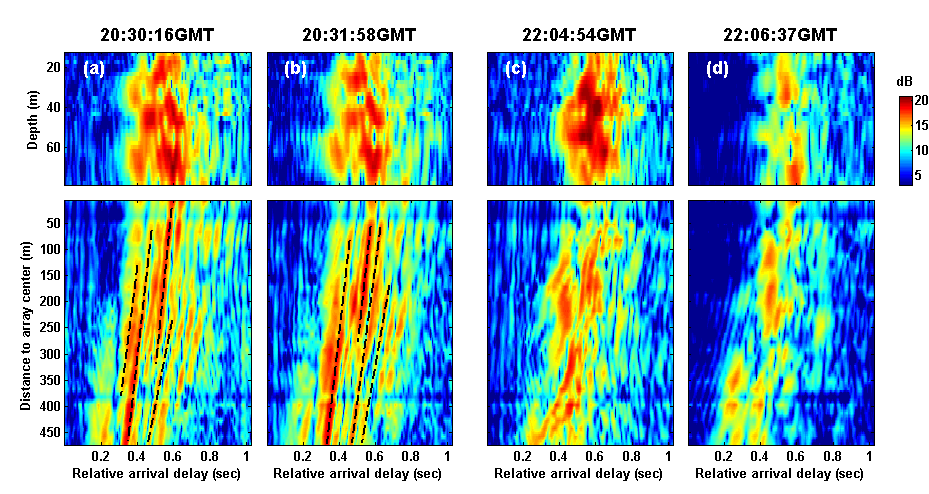
\includegraphics[width=0.75\textwidth]{jasa3.png}
%  \caption{Received acoustic intensity on the Shark VHLA during two geotimes within the $T_{g1}$ and $T_{g2}$ periods. Upper panel shows the acoustic field on the VLA portion of the array while the lower panel shows the HLA portion. (a) Tg = 20:30:16 GMT, (b) Tg = 20:31:58 GMT, (c) Tg = 22:04:54 GMT, (d) Tg = 22:06:37 GMT.}\label{fig:jasa3}
%\end{figure}
%
%Next, we show the acoustic signal arrival on the Shark VHLA during
%the two periods $T_{g1}$ and $T_{g2}$. In order to show the intensity
%variations, we show the arrival of two different LFM pings on the
%array at geotimes separated by 102 sec. In Fig.\ref{fig:jasa3}, the upper
%panel shows the acoustic signal on the VLA at 20:30:16 GMT while the
%lower panel shows the same signal arriving on the HLA. Figure 3(b)
%shows the same two arrays at 20:31:58 GMT. The parallel lines on the
%HLA data shown in the lower panels are due to the difference of
%arrival time on the HLA (see array configuration in Fig. 1(c)). The
%data on the VLA portion of the array shown in the upper panels best
%represent the modal arrivals. Note the similarity of the intensity
%values on both vertical and the horizontal array plots in Figs. 3(a)
%and 3(b), indicating the stability of the arriving signal energy
%during $Tg_1$. During $Tg_2$ the same data format is shown. At
%22:04:54 GMT shown in Fig. 3(c), both the VLA and HLA show a drastic
%change in the arrival. The signal intensity becomes very strong;
%however, different  arrivals are mixed together and difficult to
%separate. The parallel lines on the HLA were notably distorted. At
%22:06:37 GMT shown in Fig. 3(d), the arrivals show a lack of
%structure as well as lower intensity. During the time period of $T_{g2}$,
%the ISW is occupying a large fraction of the acoustic track. Mm. 2
%shows a movie of the acoustic signal arrival on the Shark VHLA
%during the two periods $T_{g1}$ and $T_{g2}$. To further quantify these
%results, we next calculate the average intensity in geotime and
%depth for the periods, $Tg_1$ and $Tg_2$.

Figure \ref{fig:zones} showing the posiotion of the acoustic sources. (a) NRL 300Hz source was fixed at lat. $39.18^o$ long. $72.94^o$ and transmitted 7 minutes of data every half hour, (b) J15 source was deployed below R/V Sharp positioned at the front of IW Rosey (Event 50) follow the propagation of the IW. This source transmitted signals fro 15 minutes every half hour and was quite during the time when NRL source was on. This way it was assured that there were continuous transmission during the IW passage. In addition, the R/V Sharp source provided acoustic source hanging below the ship at fixed position with respect to R/V Sharp which was moving with the front of IW (at ~0.5m/s) and transmitted during the quiet periods when NRL source was down.

\subsection{Transmission from fixed source(NRL 300Hz)}
\subsubsection{20:30GMT-20:37GMT}

Figure\ref{fig:r2030} shows the radar image at 20:30GMT. The ISWs hasn't arrived
at the acoustic path - about 4km away at the closest point (SHARK
VLA). In figure \ref{fig:a2030}, the received signal on VLA shows a 3-stripe
pattern, which, after modal decomposition (Fig\ref{fig:m2030}), can be
contributed to the very strong and steady 2nd and 3rd modes. The
modal decomposition figures also show the intensity of the 1st mode
grows around 20:36GMT. Although the fluctuation of the total
intensity is less than 2.5dB, from the modal amplitude plot, we can
see the increase of the intensity mode 1 and 4 and the decrease of
mode 2 and 3. The energy exchange among the different modes here
suggest the occurrence of the modal coupling.
%\begin{figure}[H]
 % \centering
  %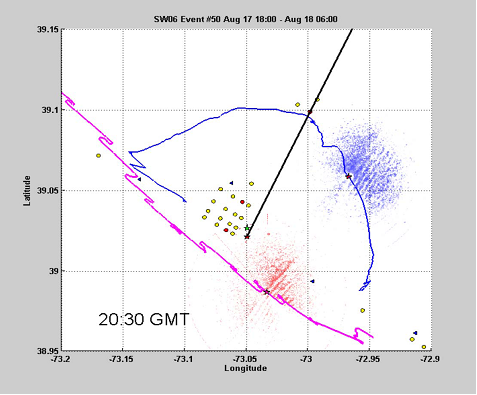
\includegraphics[width=0.5\textwidth]{radar2030.png}
  %\caption{Radar image of ISW at 20:30GMT}\label{fig:r2030}
%\end{figure}
%
%\begin{figure}
%  \centering
%  \begin{tabular}{l}
%  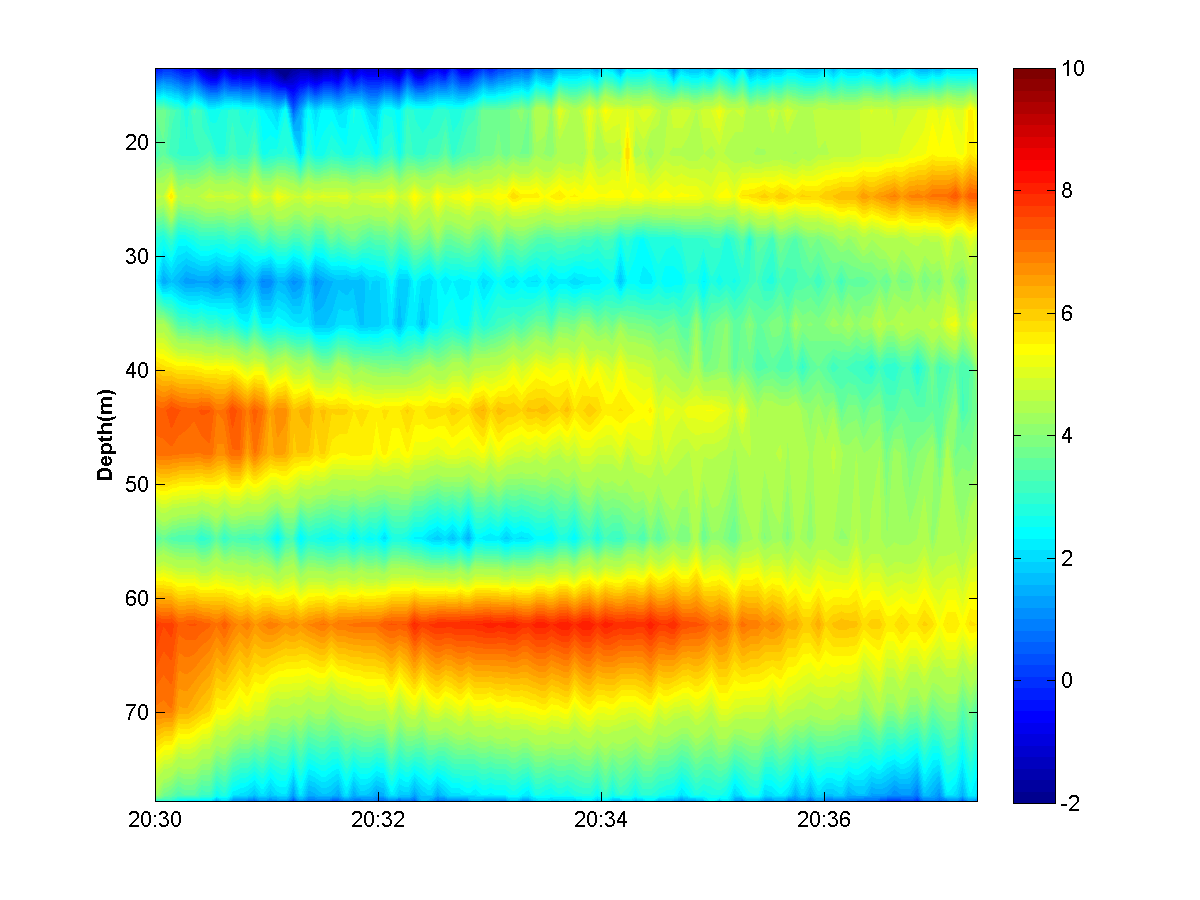
\includegraphics[width=0.5\textwidth,height=0.2\textwidth]{0817_2030_vla.png}\\
%  \ 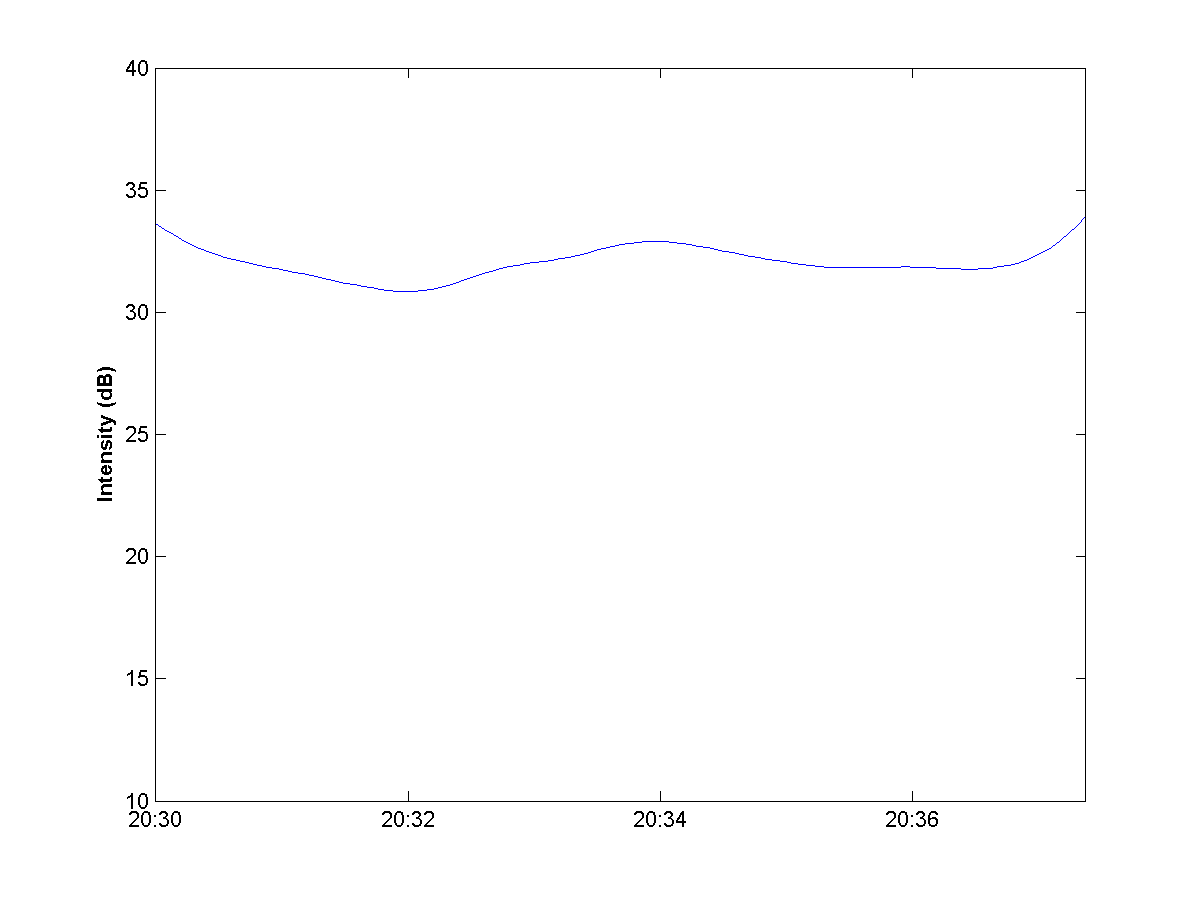
\includegraphics[width=0.44\textwidth,height=0.2\textwidth]{0817_2030_eng.png}\\
%  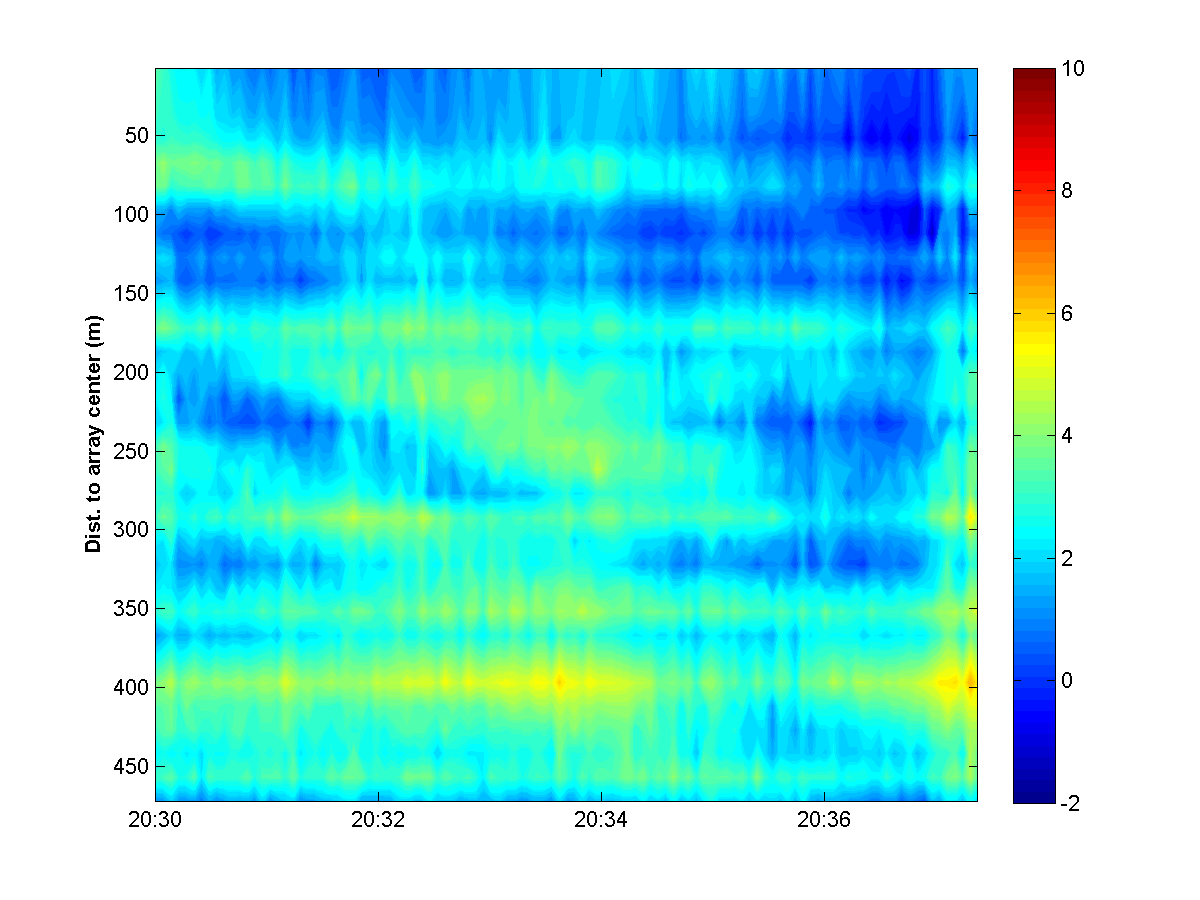
\includegraphics[width=0.5\textwidth,height=0.2\textwidth]{0817_2030_hla.png}\\
%  \end{tabular}
%  \caption{Received signal on Shark VLA (top), HLA (bottom) and signal intensity (middle) from Aug.17 20:30GMT to 20:37GMT }\label{fig:a2030}
%\end{figure}

%\begin{figure}
 % \centering
 % \begin{tabular}{lrr}
 % 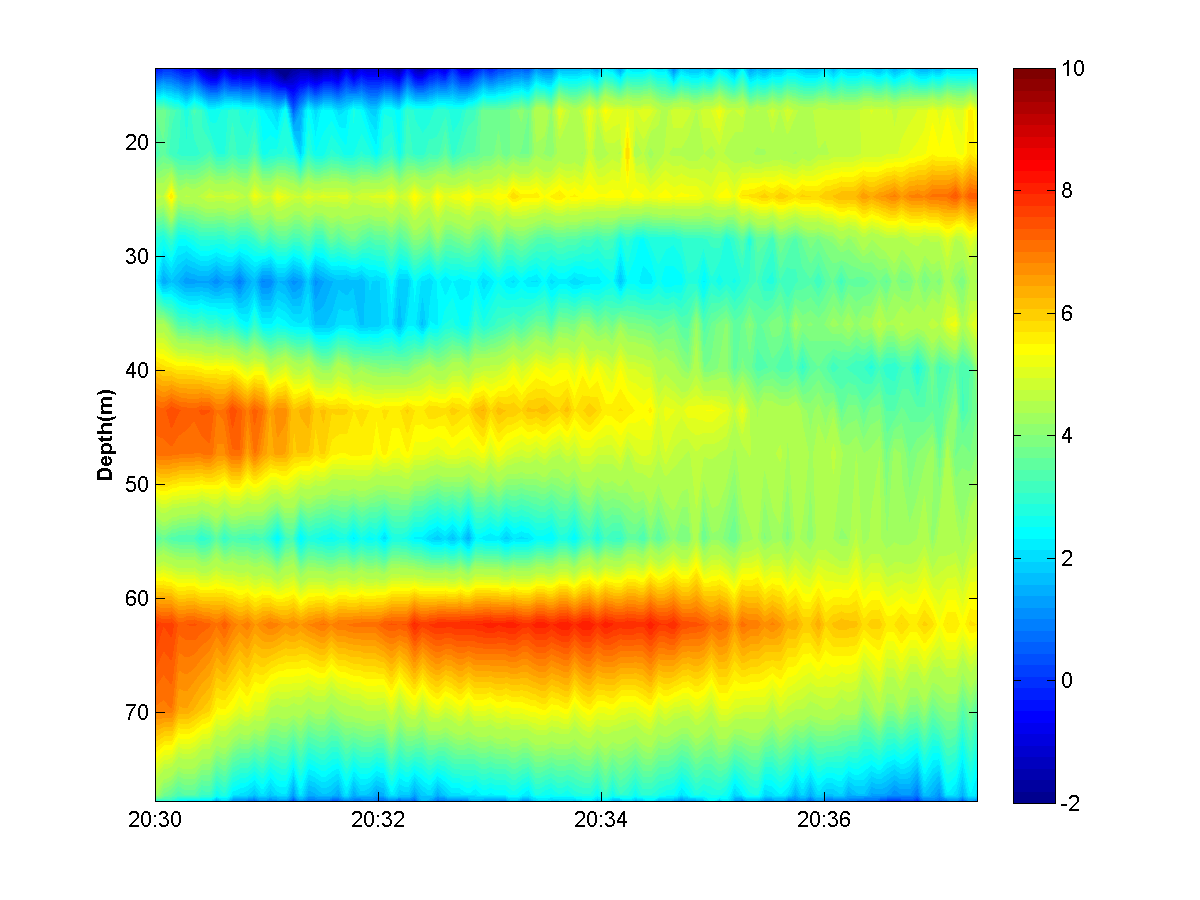
\includegraphics[width=0.3\textwidth,height=0.1\textwidth]{0817_2030_vla.png}
 % 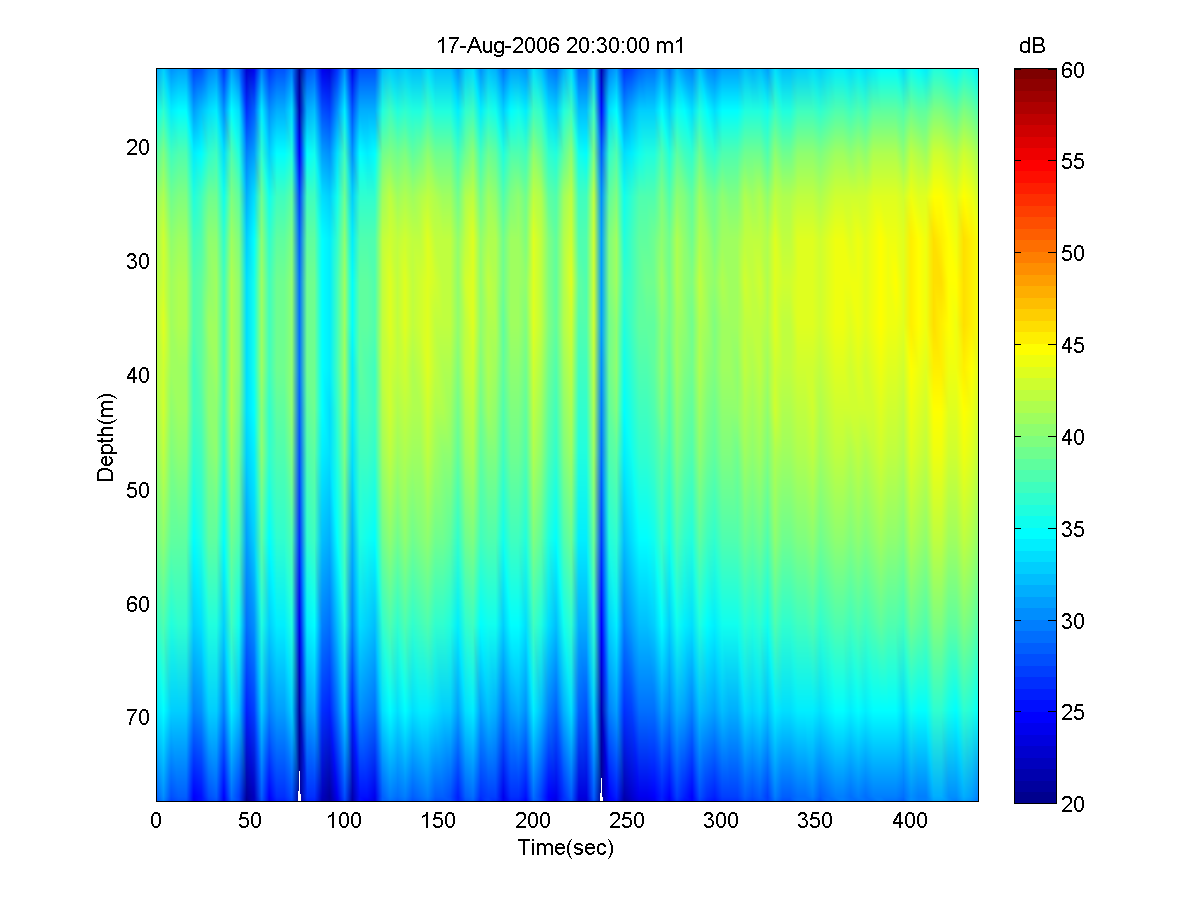
\includegraphics[width=0.3\textwidth,height=0.1\textwidth]{nrl_200608172030_m1.png}
 % 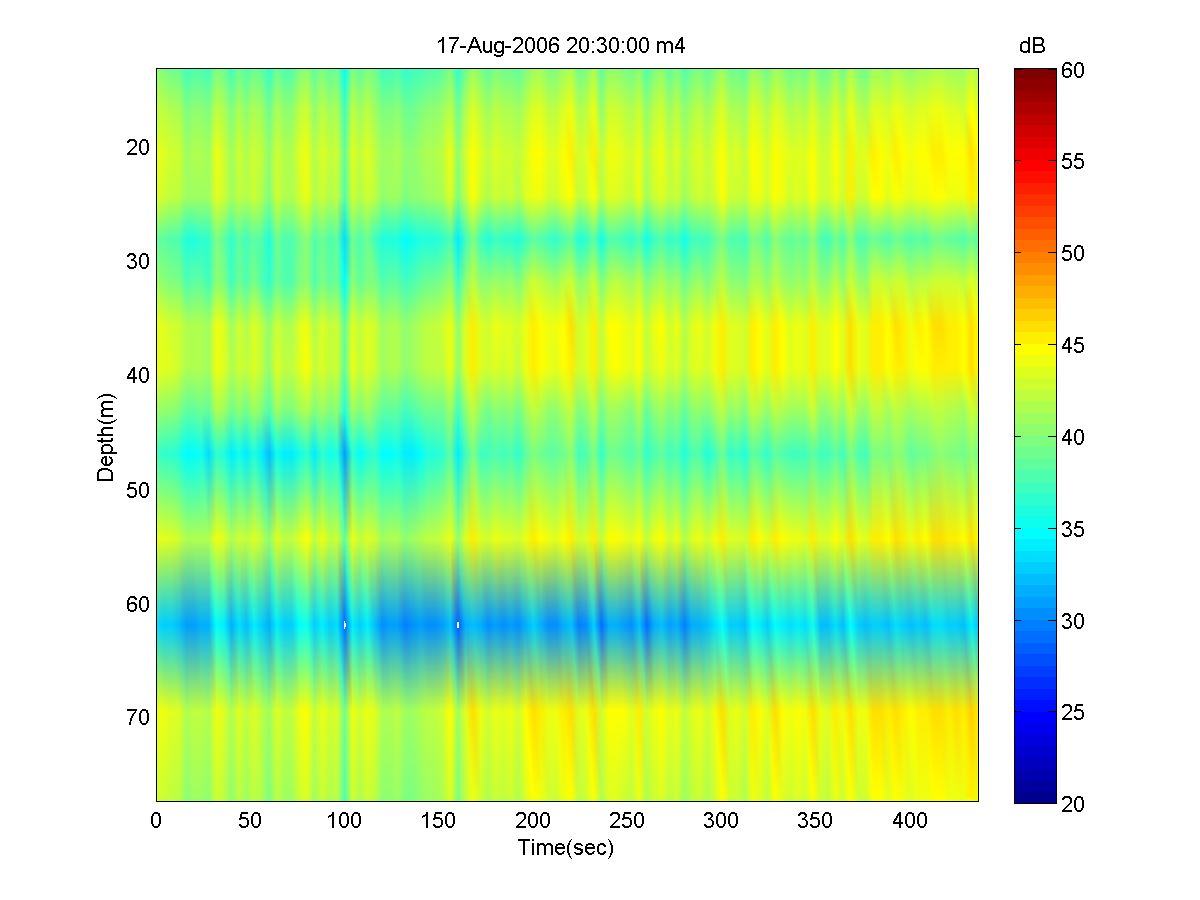
\includegraphics[width=0.3\textwidth,height=0.1\textwidth]{nrl_200608172030_m4.png}\\
 % 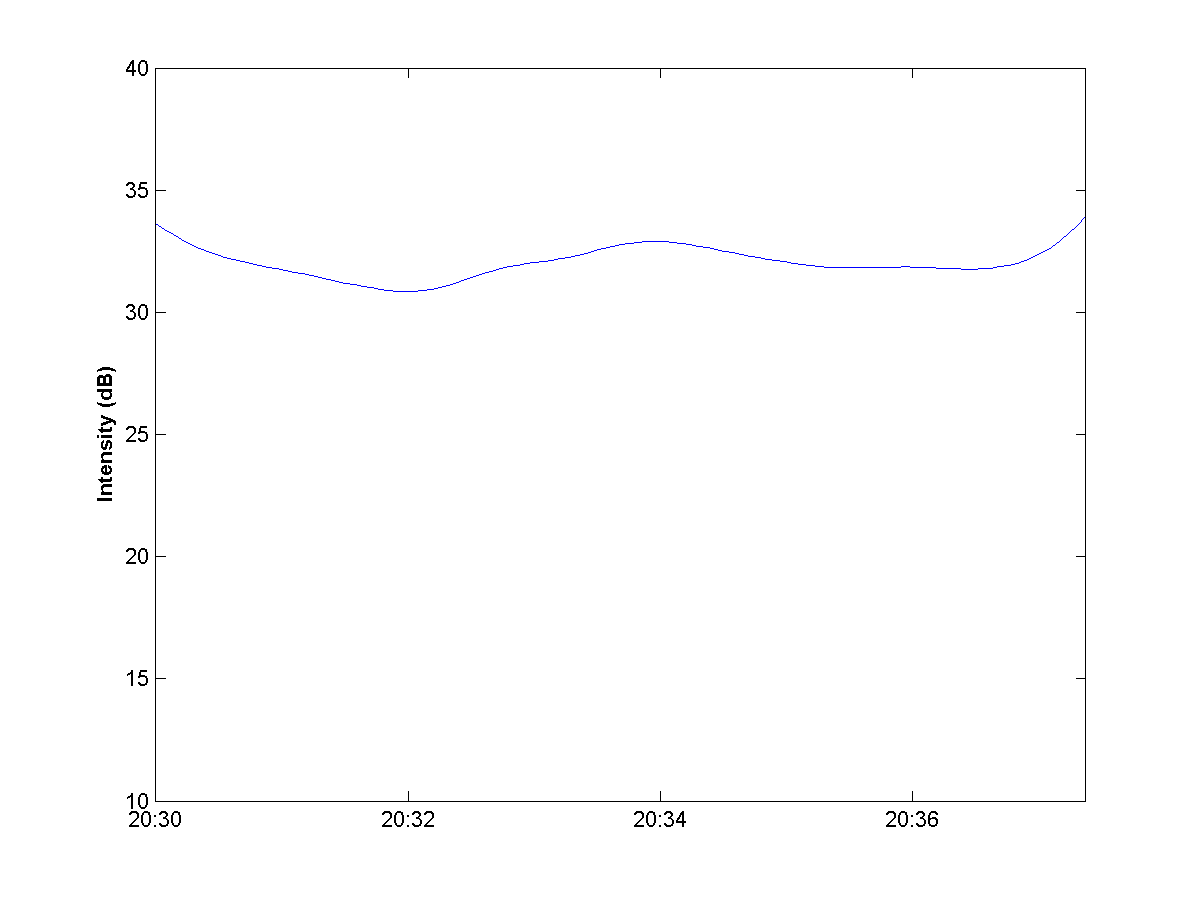
\includegraphics[width=0.3\textwidth,height=0.1\textwidth]{0817_2030_eng.png}
 % 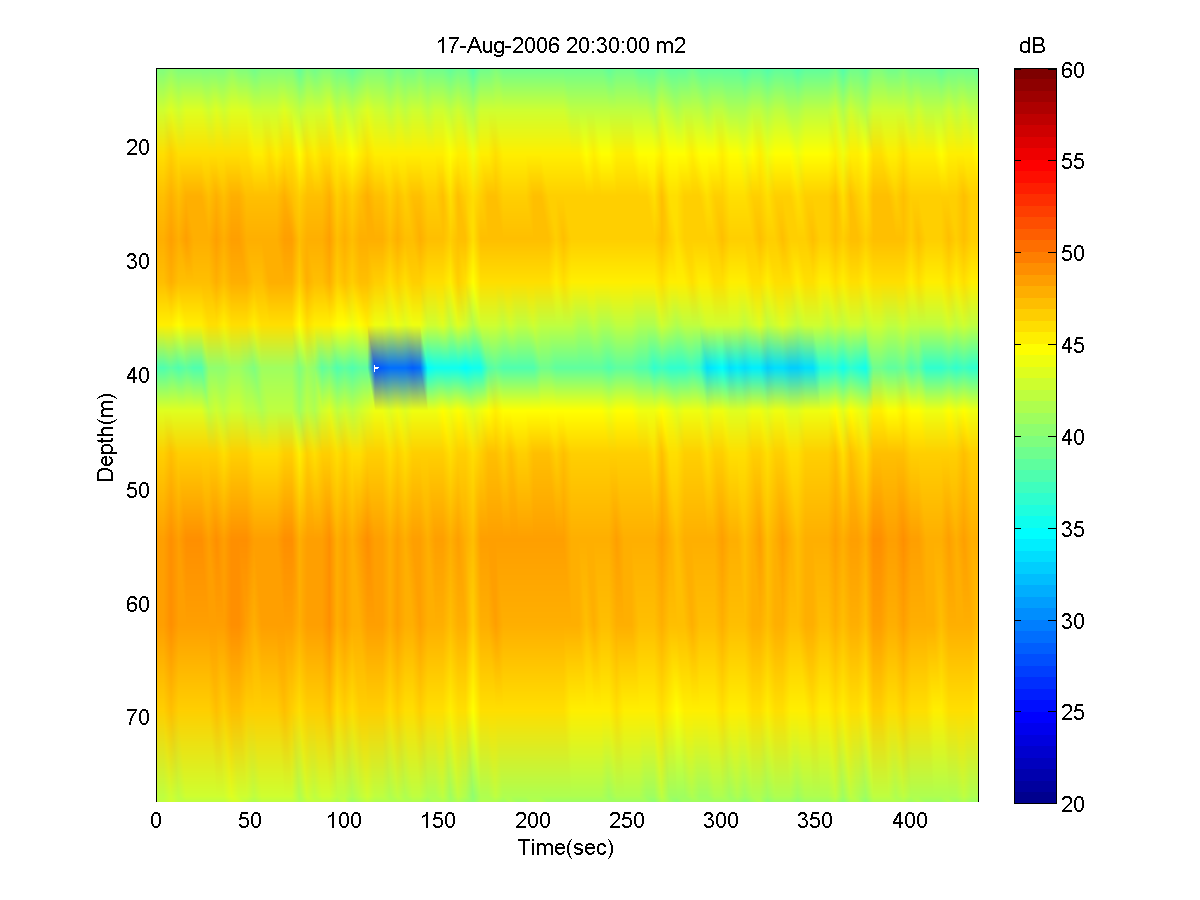
\includegraphics[width=0.3\textwidth,height=0.1\textwidth]{nrl_200608172030_m2.png}
  %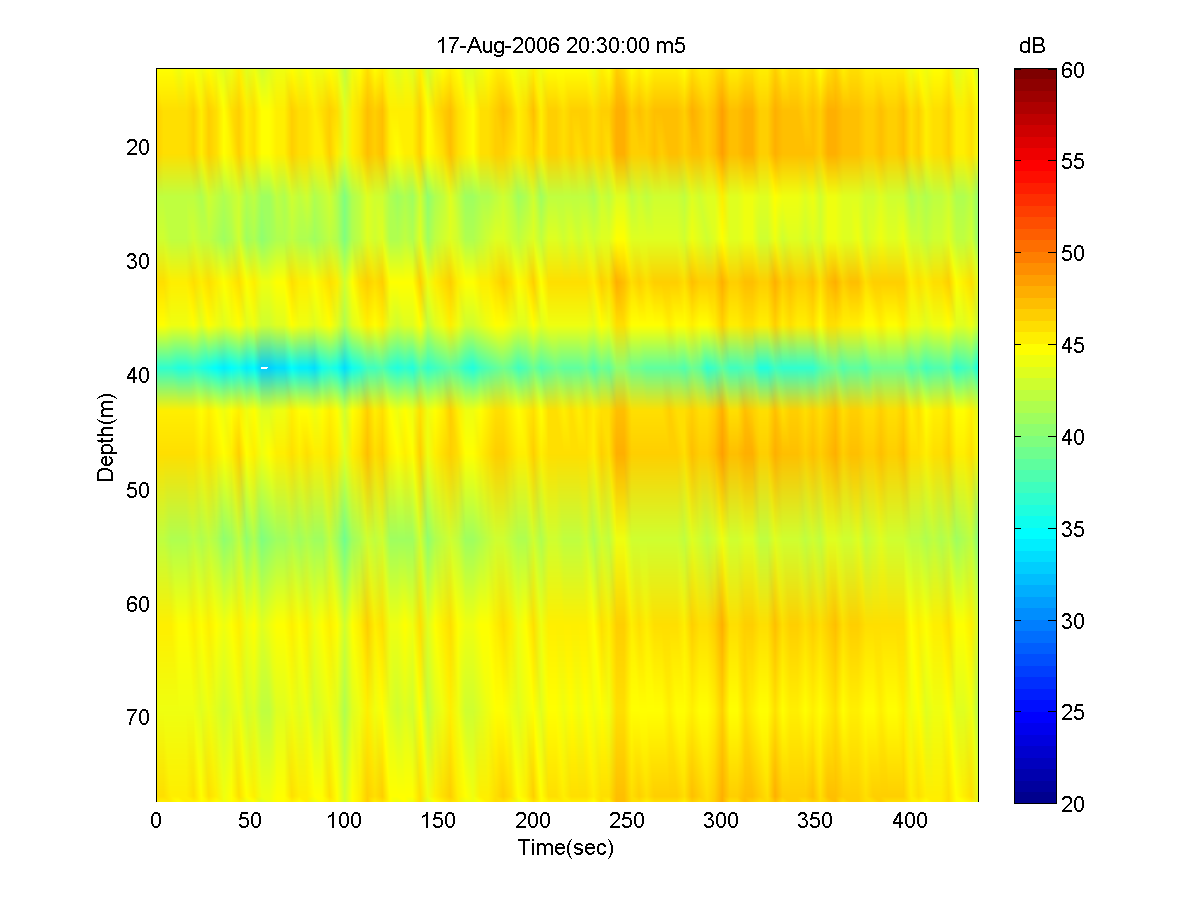
\includegraphics[width=0.3\textwidth,height=0.1\textwidth]{nrl_200608172030_m5.png}\\
  %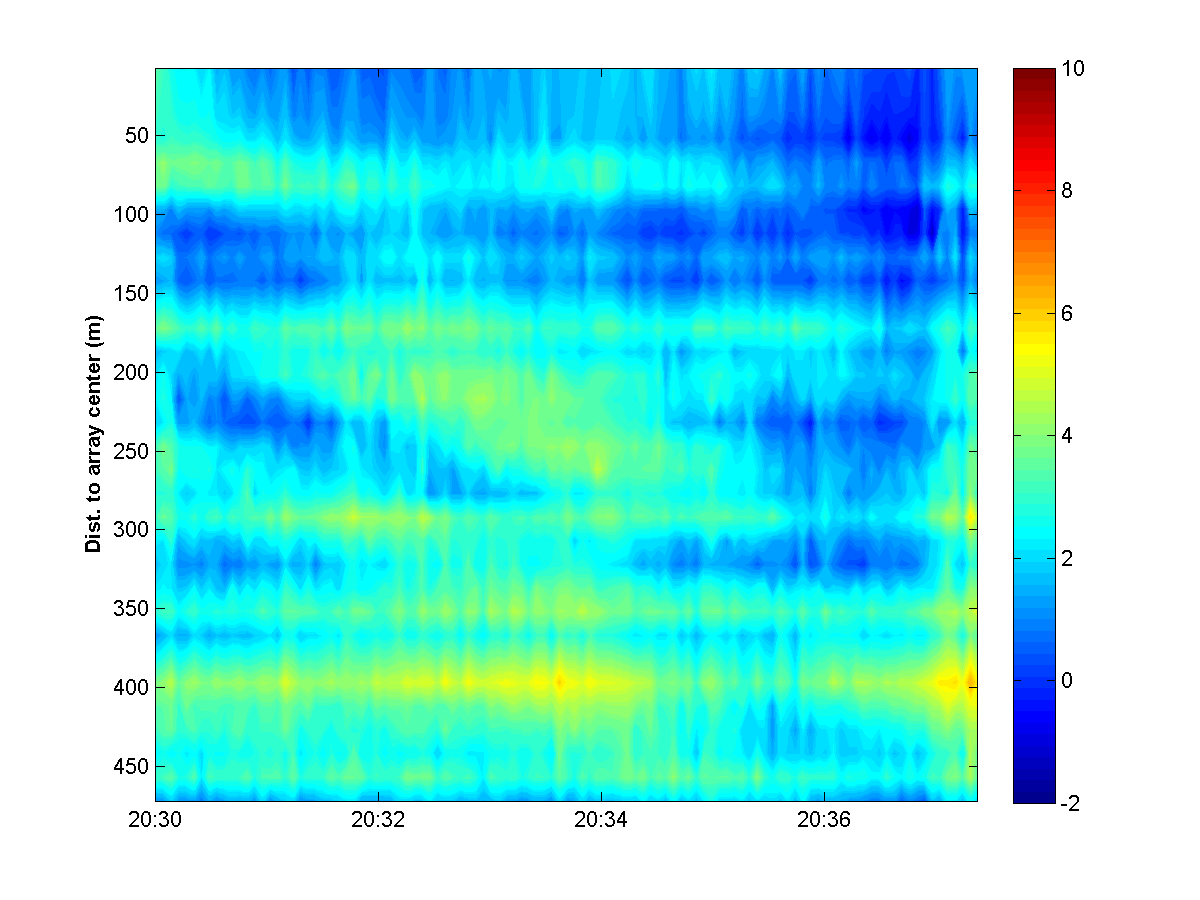
\includegraphics[width=0.3\textwidth,height=0.1\textwidth]{0817_2030_hla.png}
  %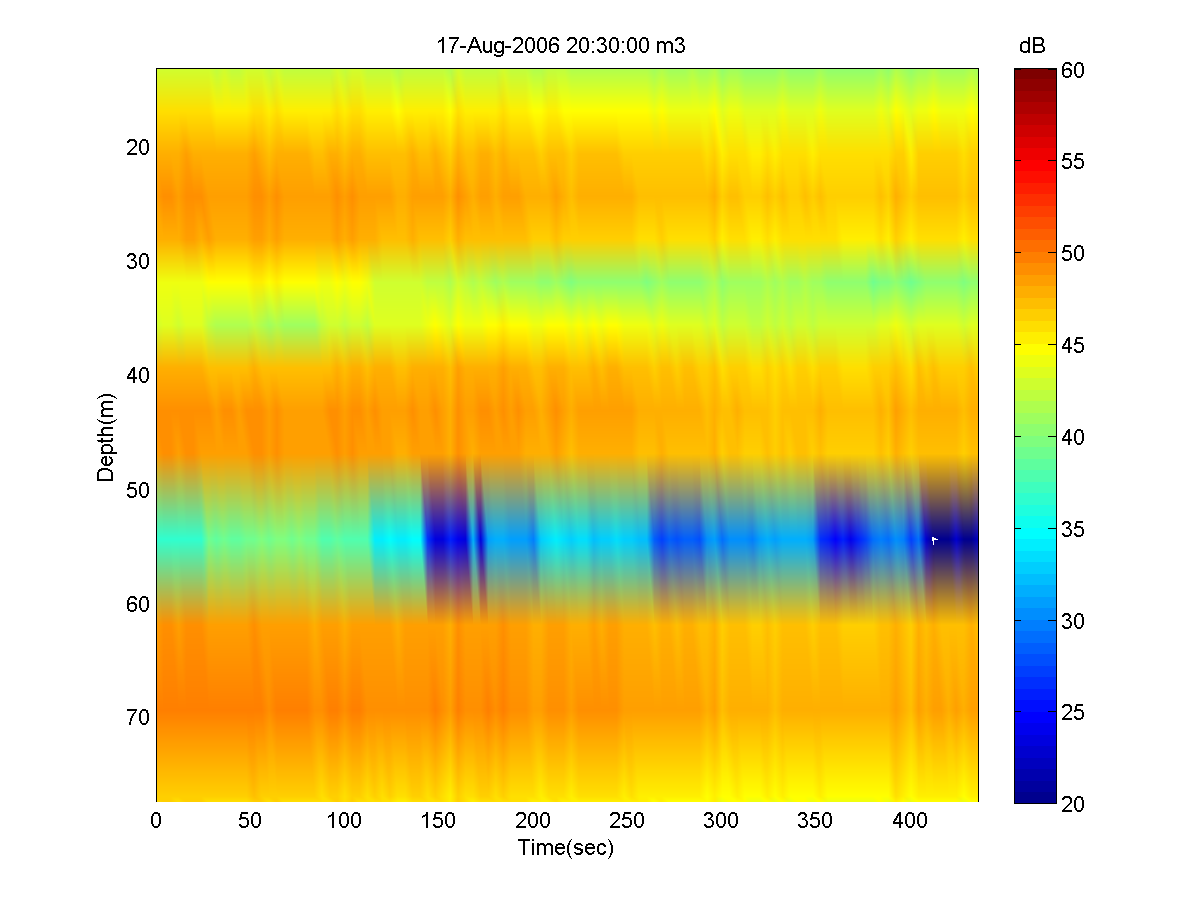
\includegraphics[width=0.3\textwidth,height=0.1\textwidth]{nrl_200608172030_m3.png}
  %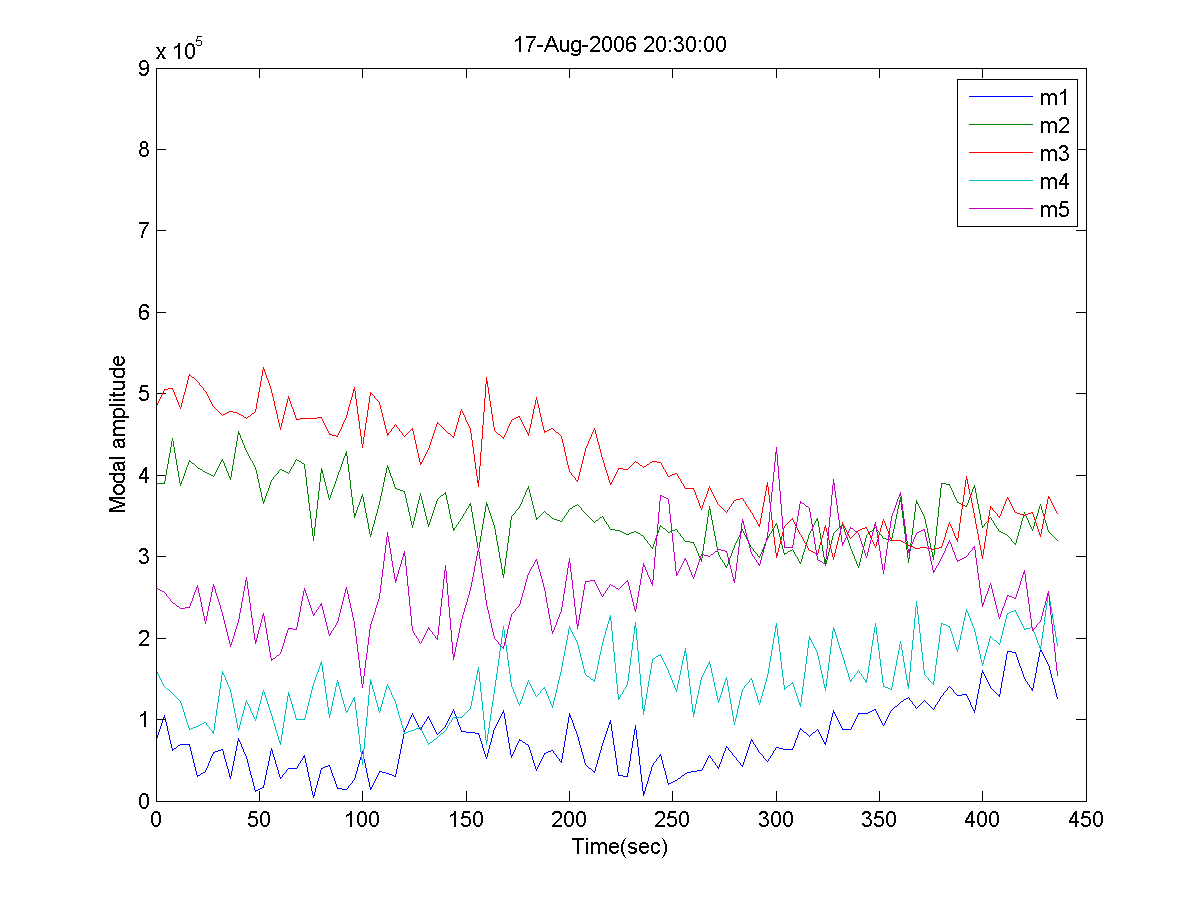
\includegraphics[width=0.3\textwidth,height=0.1\textwidth]{nrl_ma_200608172030.png}\\
 % \end{tabular}
  %\caption{Received signal on Shark array from Aug.17 20:30GMT to 20:37GMT. Left column, from top to bottom: signal on VLA, VLA signal intensity, signal on HLA; middle column: mode 1-3; right column: mode 4, 5, and modal amplitudes.}\label{fig:m2030}
%\end{figure}


\subsubsection{21:00GMT-21:07GMT}

Figure\ref{fig:r2100} shows the radar image at 21:00GMT. The ISWs is still about
1km away from the VLA, and very similar to the previous time period
(20:30GMT - 20:37GMT), only very little fluctuation of the total
intensity is shown (Fig.\ref{fig:a2100}). On the modal decomposition plot (Fig.\ref{fig:m2100}), the 3rd mode
grows while the other modes decrease to various extends. The modal
coupling might cause this as well.

%\begin{figure}[H]
 % \centering
  %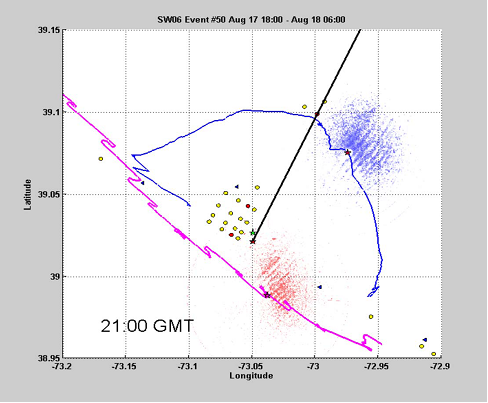
\includegraphics[width=0.5\textwidth]{radar2100.png}
 % \caption{Radar image of ISW at 21:00GMT}\label{fig:r2100}
%\end{figure}
%
%\begin{figure}[H]
%  \centering
%  \begin{tabular}{l}
%  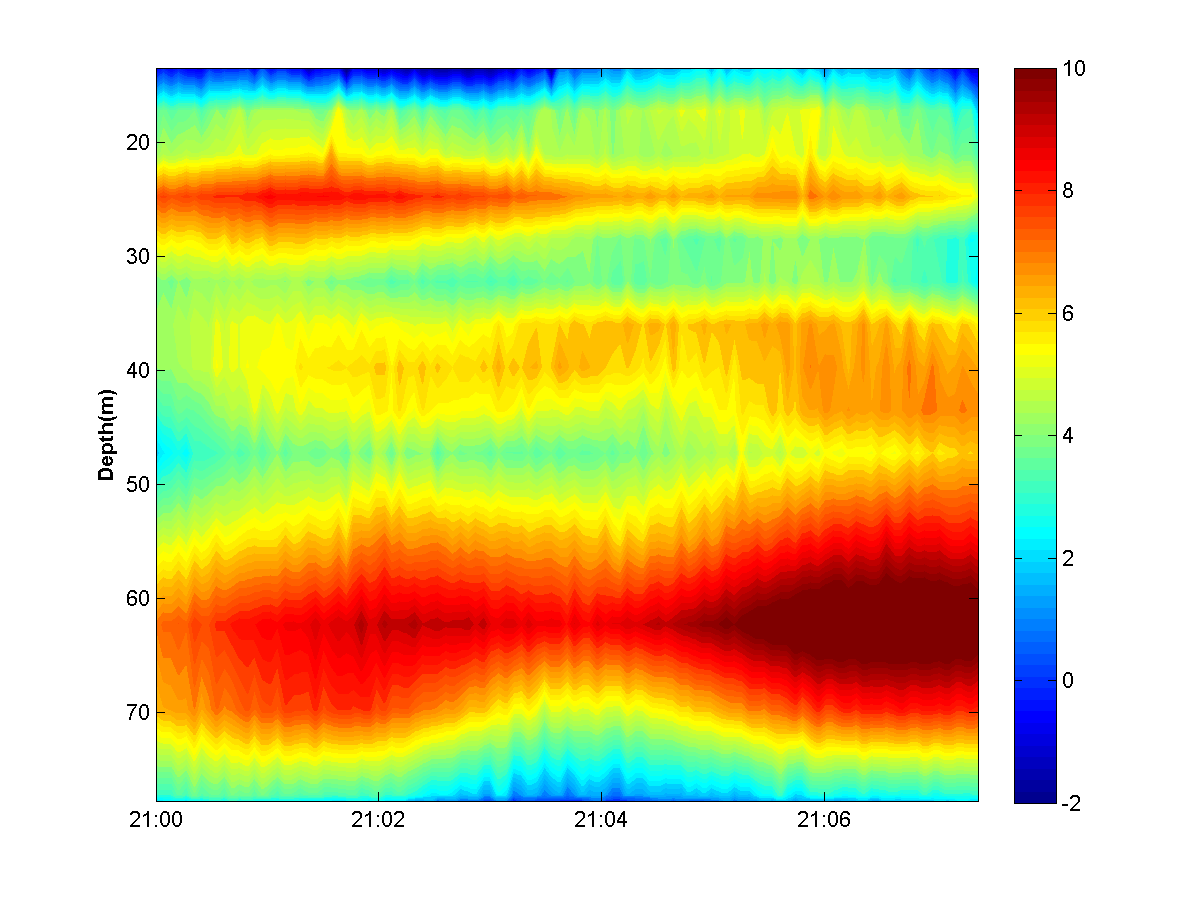
\includegraphics[width=0.5\textwidth,height=0.2\textwidth]{0817_2100_vla.png}\\
%  \ 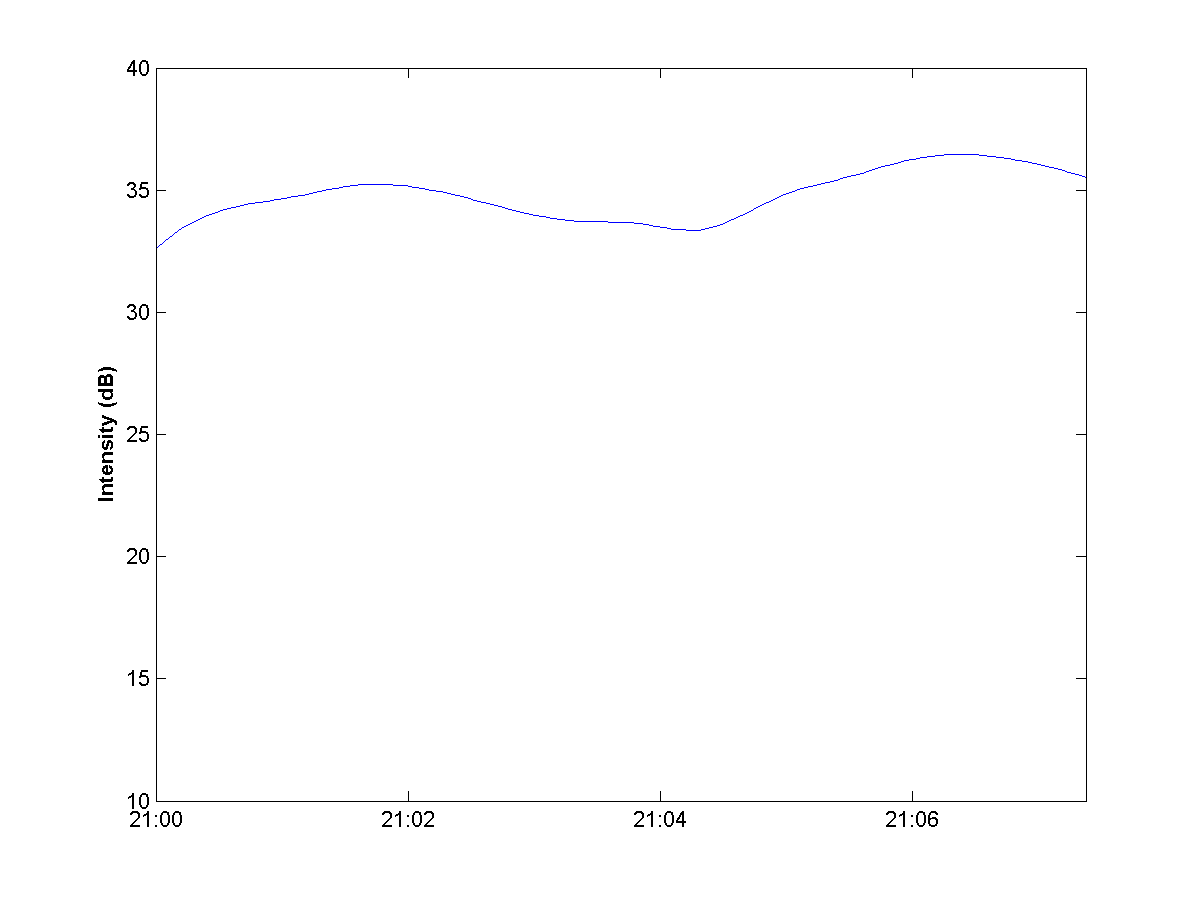
\includegraphics[width=0.44\textwidth,height=0.2\textwidth]{0817_2100_eng.png}\\
%  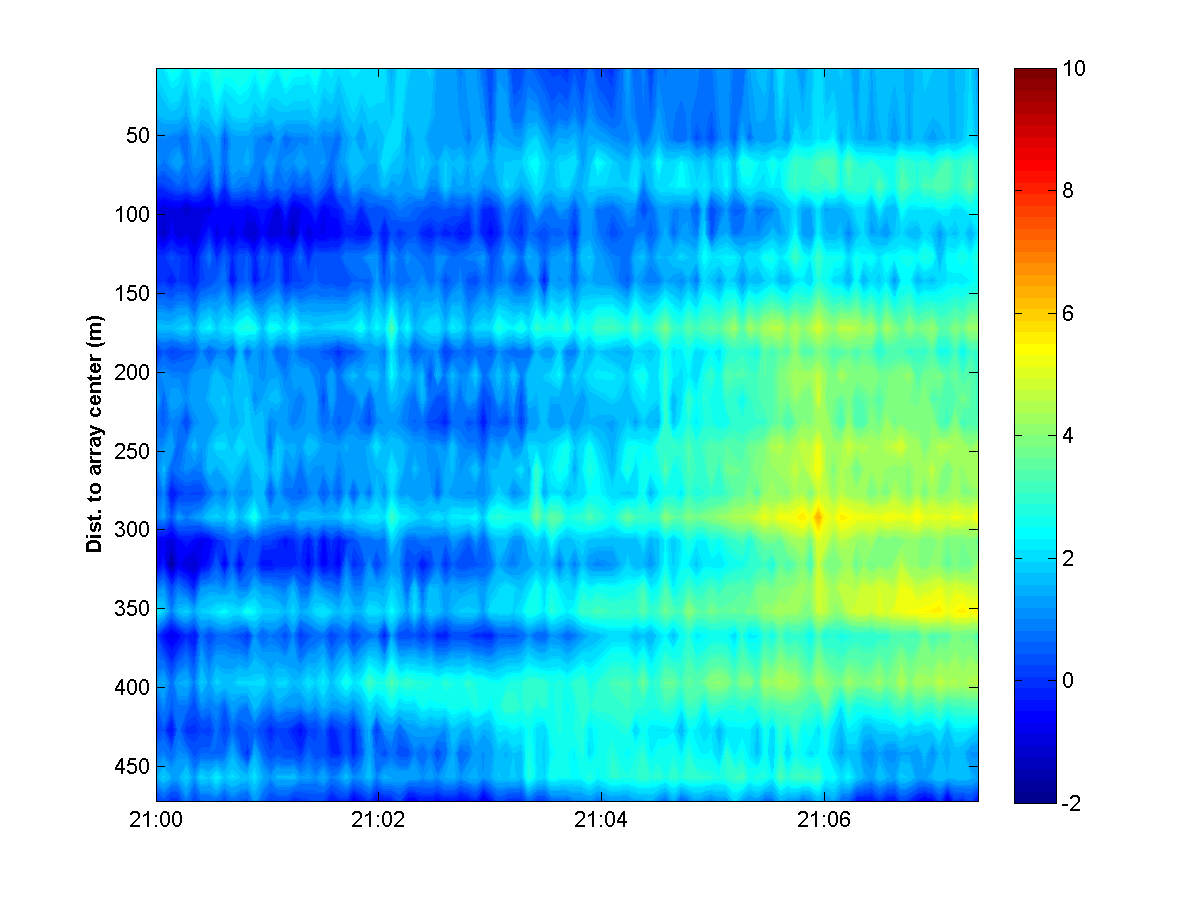
\includegraphics[width=0.5\textwidth,height=0.2\textwidth]{0817_2100_hla.png}\\
%  \end{tabular}
%  \caption{Received signal on Shark VLA (top), HLA (bottom) and signal intensity (middle) from Aug.17 21:00GMT to 21:07GMT }\label{fig:a2100}
%\end{figure}
%
%\begin{figure}[H]
%  \centering
%  \begin{tabular}{cc}
%  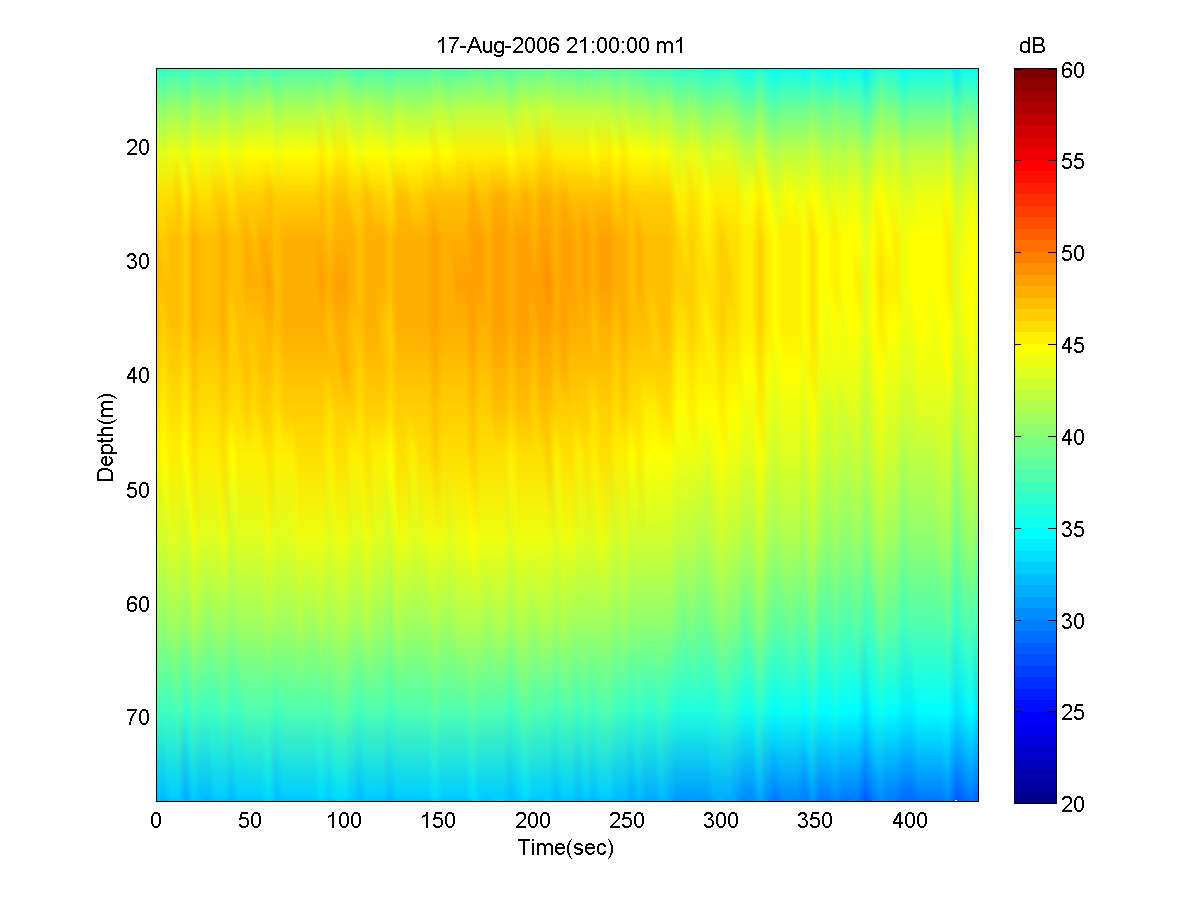
\includegraphics[width=0.5\textwidth,height=0.2\textwidth]{nrl_200608172100_m1.png}
%  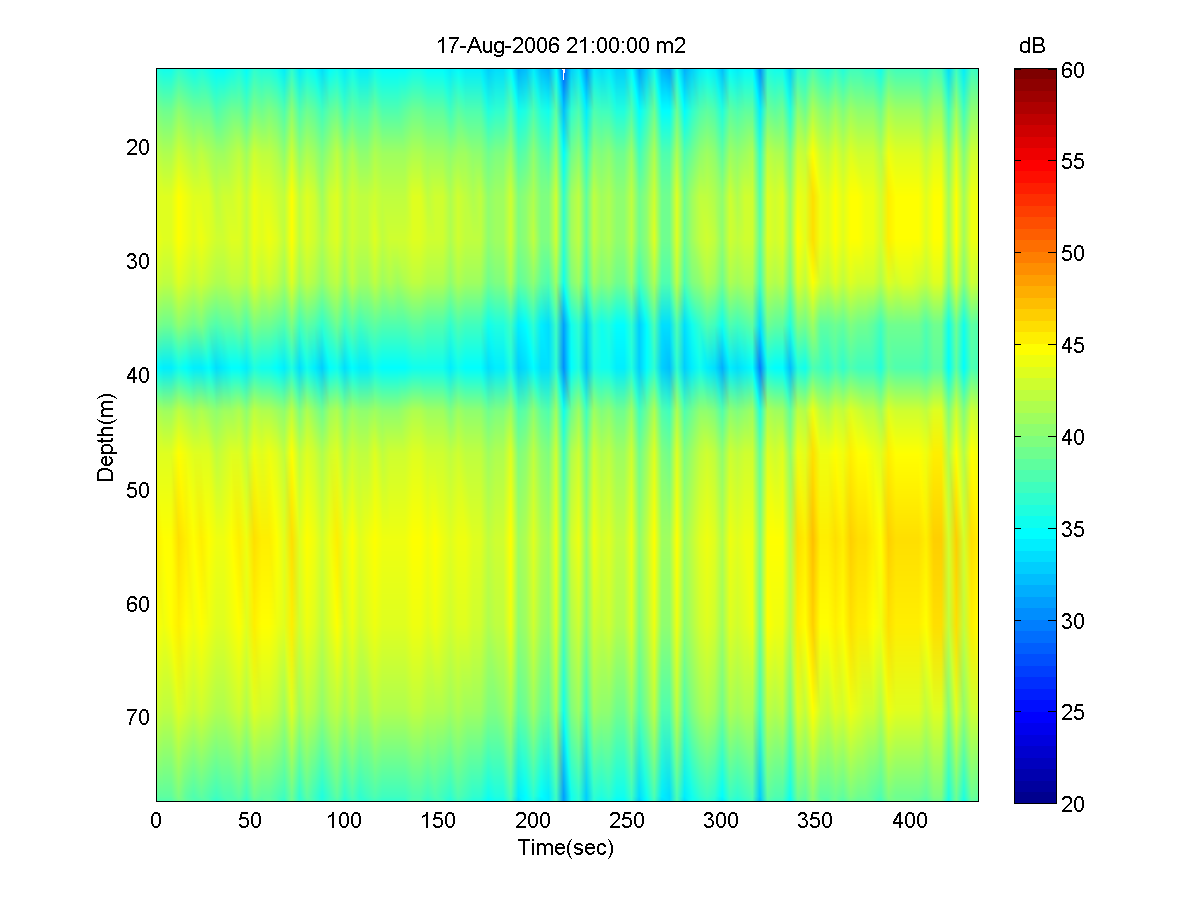
\includegraphics[width=0.5\textwidth,height=0.2\textwidth]{nrl_200608172100_m2.png}\\
%  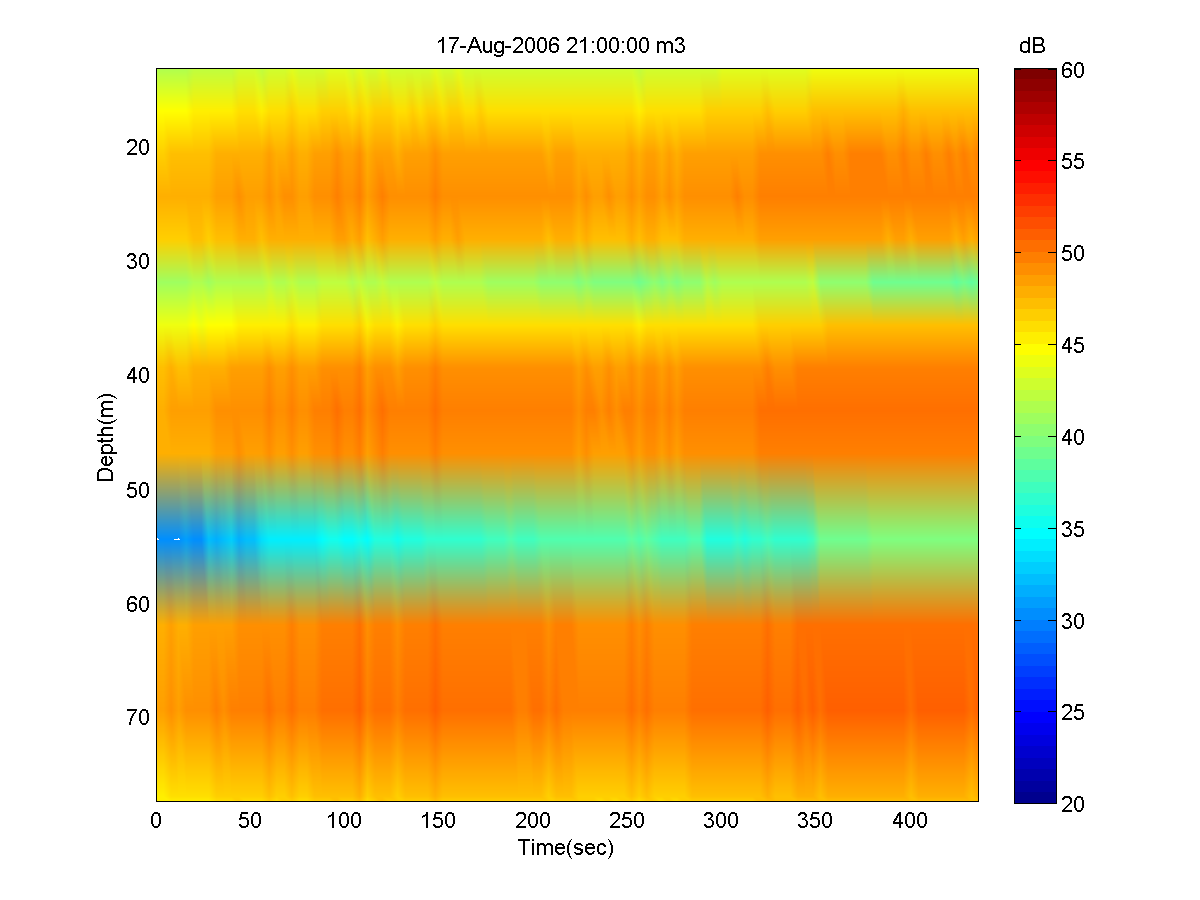
\includegraphics[width=0.5\textwidth,height=0.2\textwidth]{nrl_200608172100_m3.png}
%  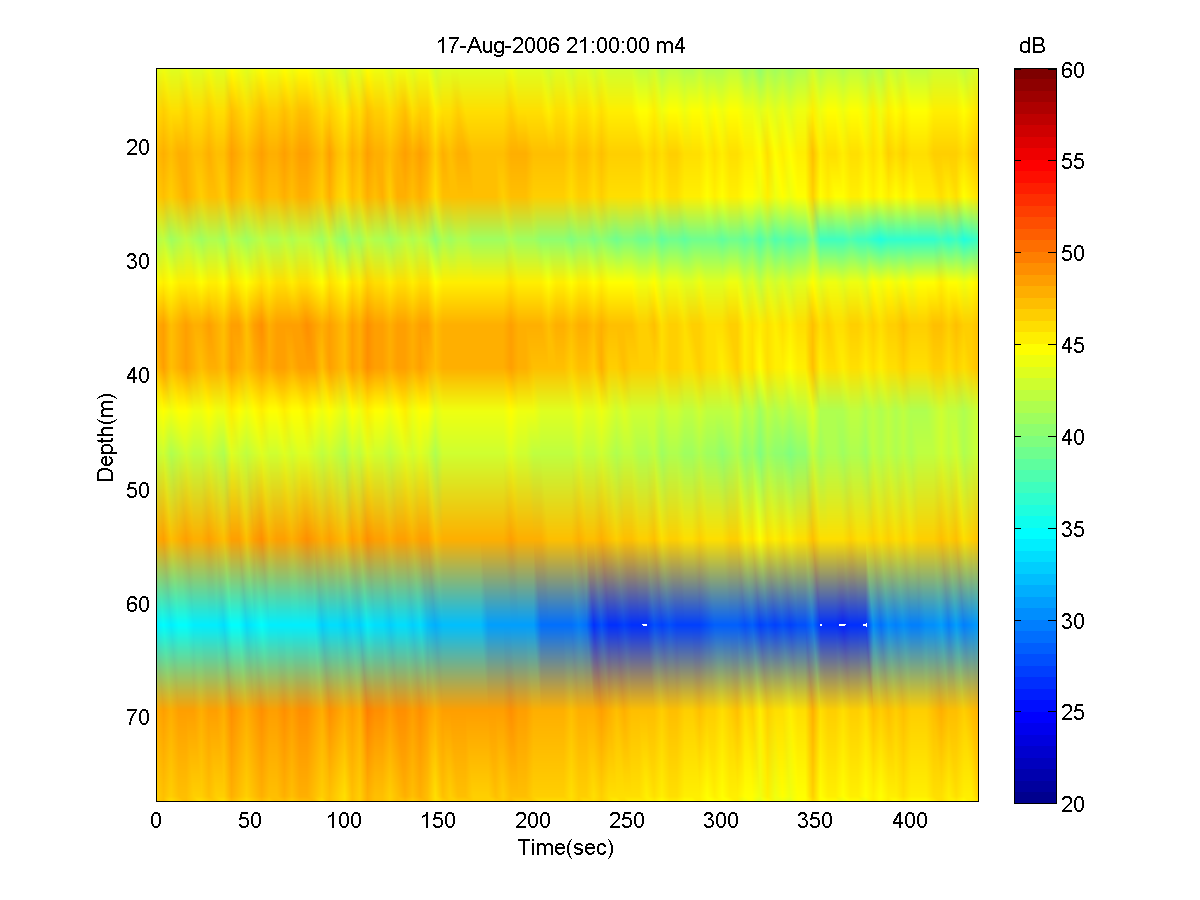
\includegraphics[width=0.5\textwidth,height=0.2\textwidth]{nrl_200608172100_m4.png}\\
%  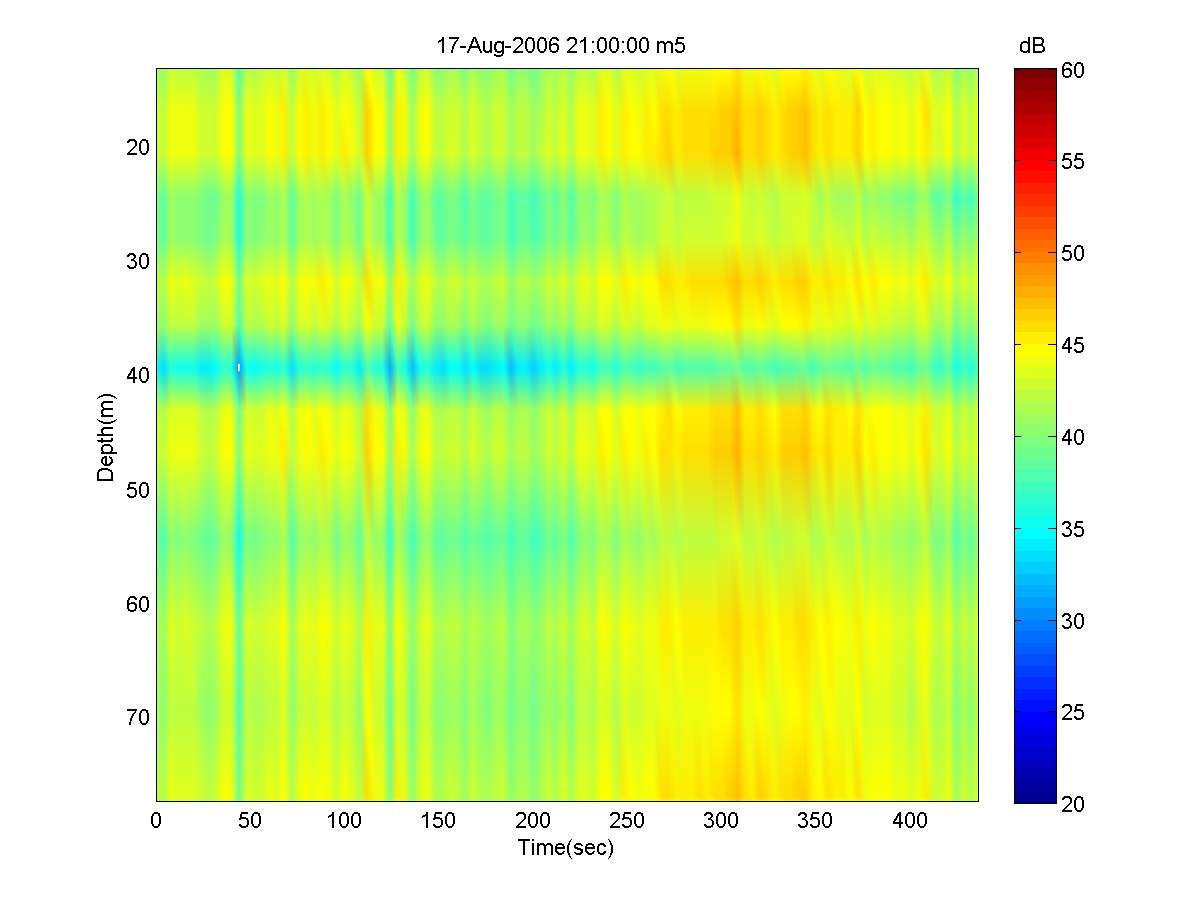
\includegraphics[width=0.5\textwidth,height=0.2\textwidth]{nrl_200608172100_m5.png}
%  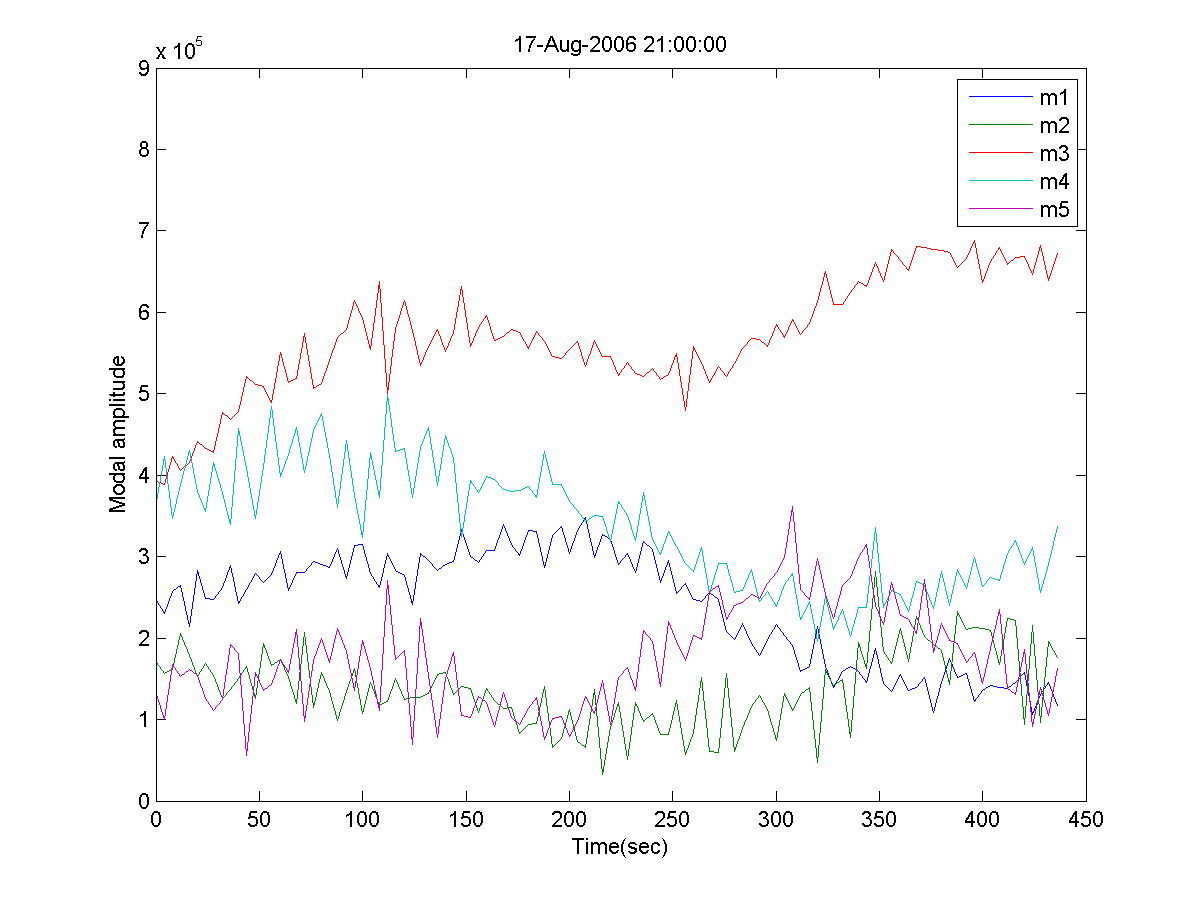
\includegraphics[width=0.5\textwidth,height=0.2\textwidth]{nrl_ma_200608172100.png}\\
%  \end{tabular}
%  \caption{Modal decomposition and amplitude of the signal received on Shark VLA from Aug.17 21:00GMT to 21:07GMT }\label{fig:m2100}
%\end{figure}


%\begin{figure}
 % \centering
  %\begin{tabular}{lrr}
  %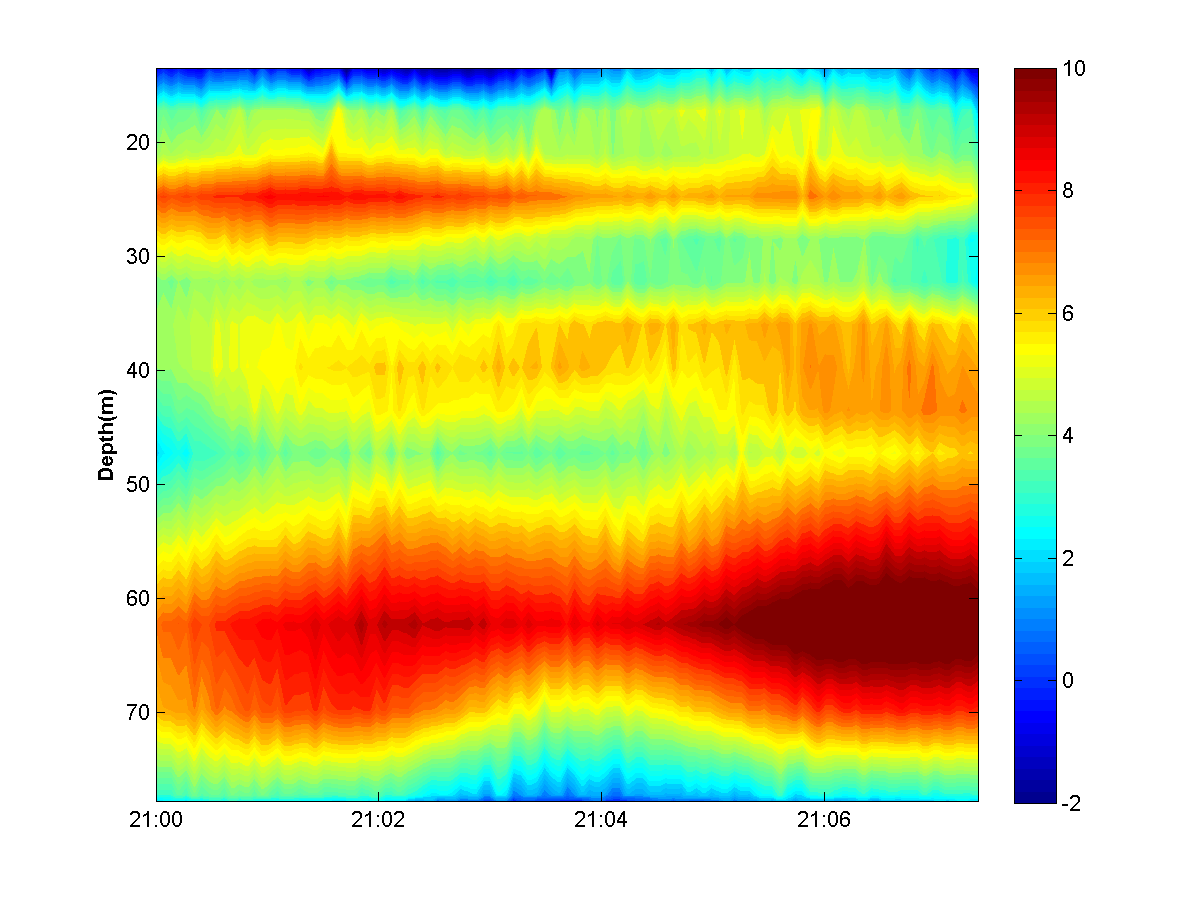
\includegraphics[width=0.3\textwidth,height=0.1\textwidth]{0817_2100_vla.png}
  %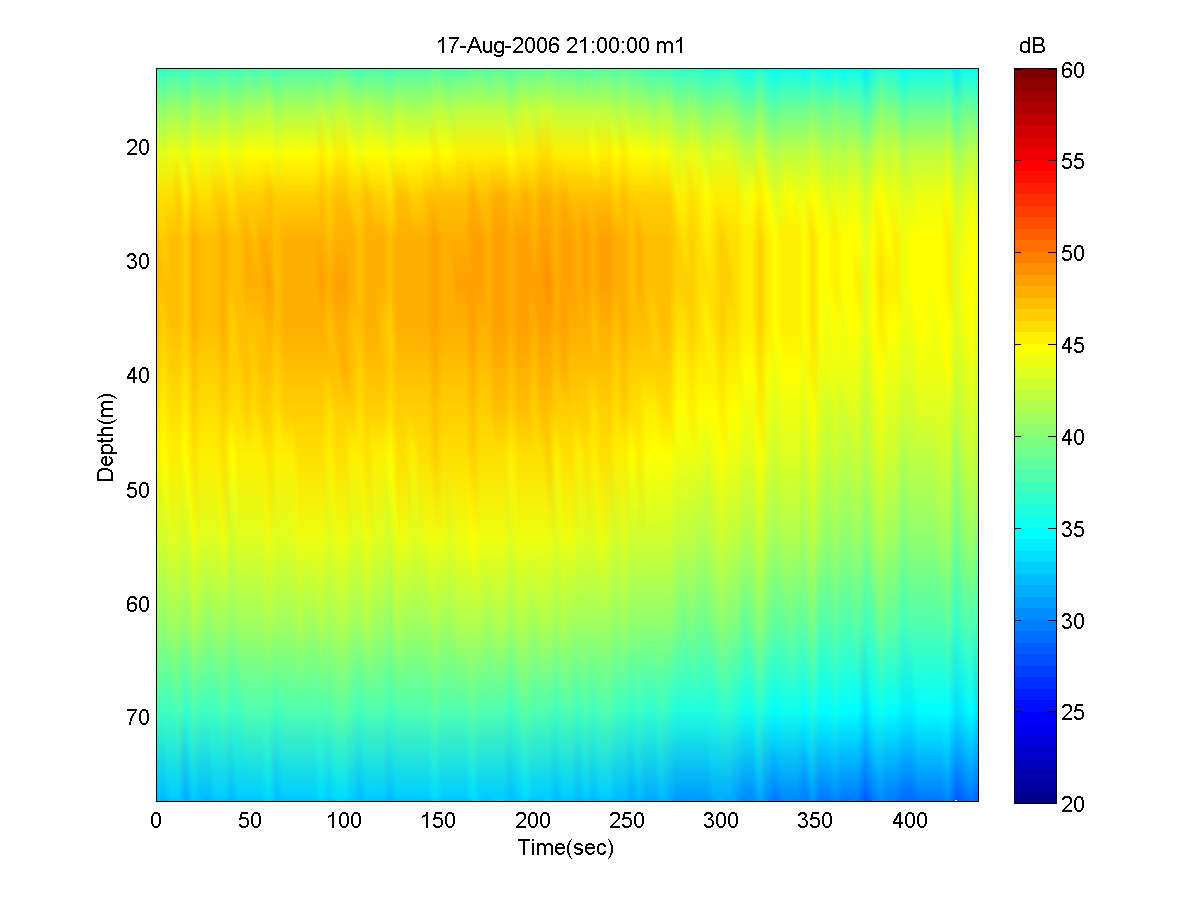
\includegraphics[width=0.3\textwidth,height=0.1\textwidth]{nrl_200608172100_m1.png}
  %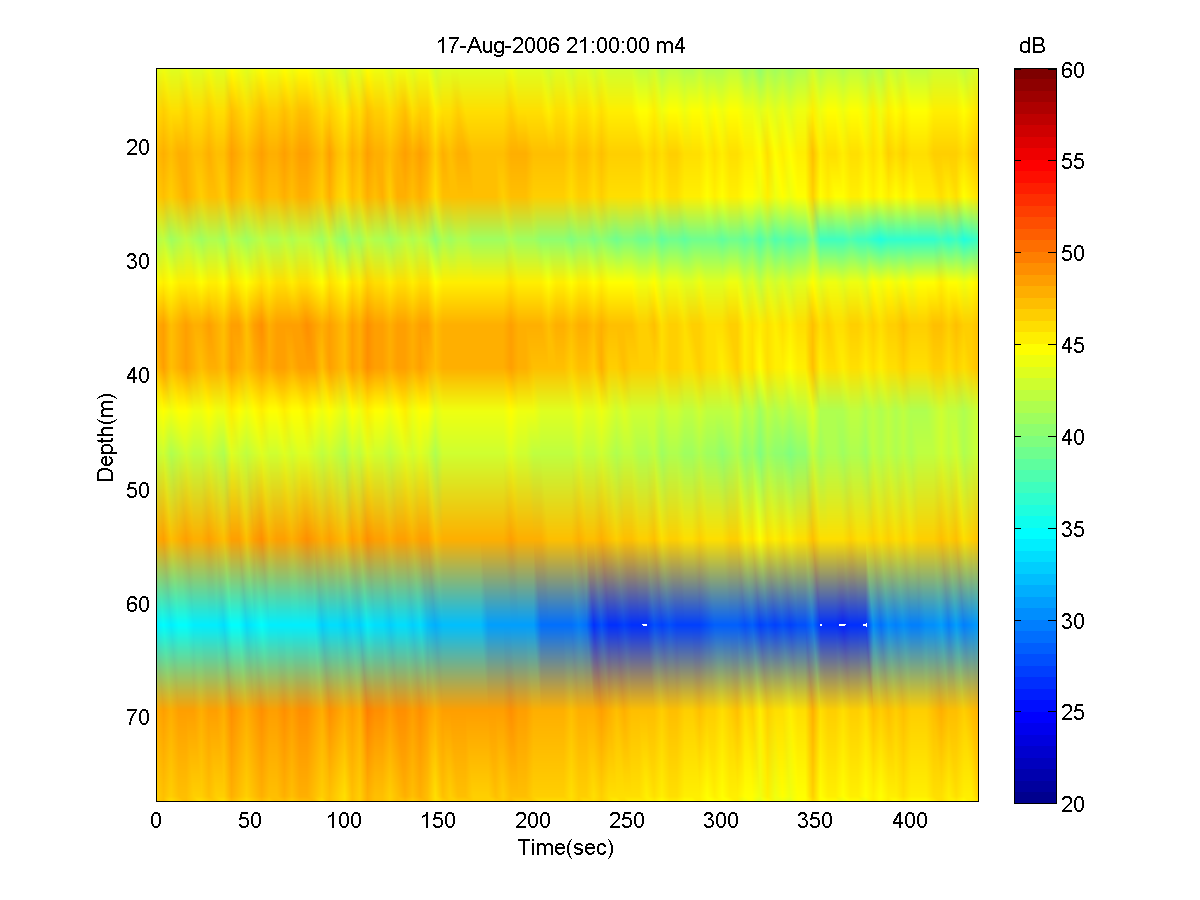
\includegraphics[width=0.3\textwidth,height=0.1\textwidth]{nrl_200608172100_m4.png}\\
  %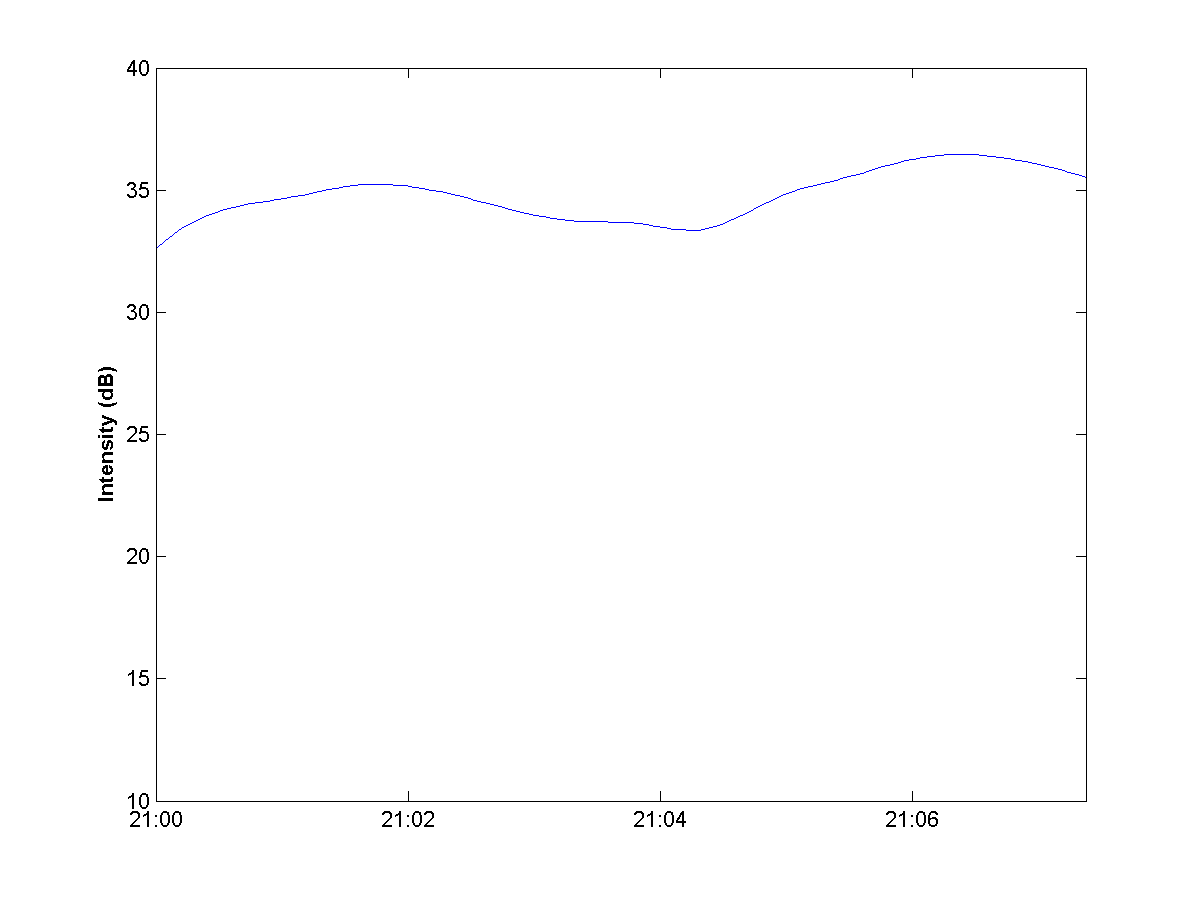
\includegraphics[width=0.3\textwidth,height=0.1\textwidth]{0817_2100_eng.png}
  %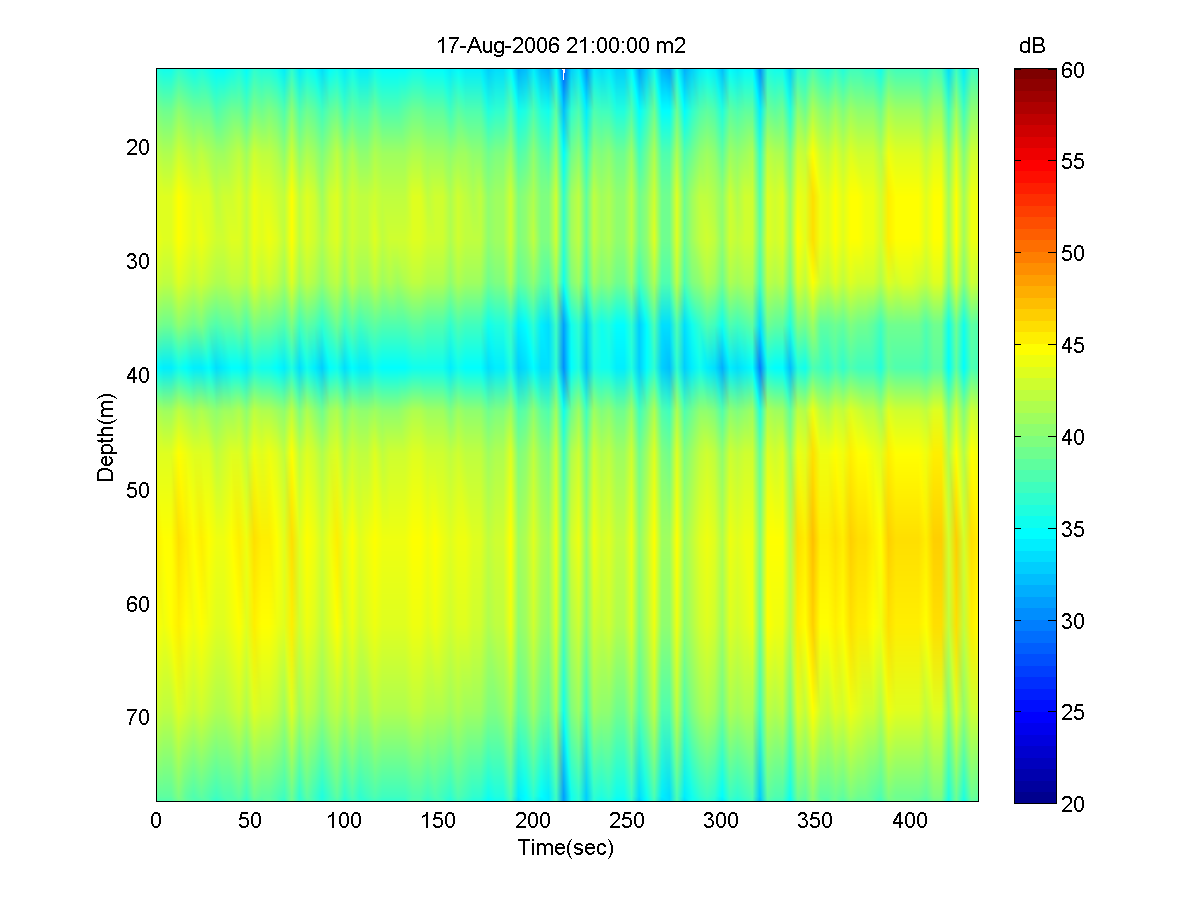
\includegraphics[width=0.3\textwidth,height=0.1\textwidth]{nrl_200608172100_m2.png}
  %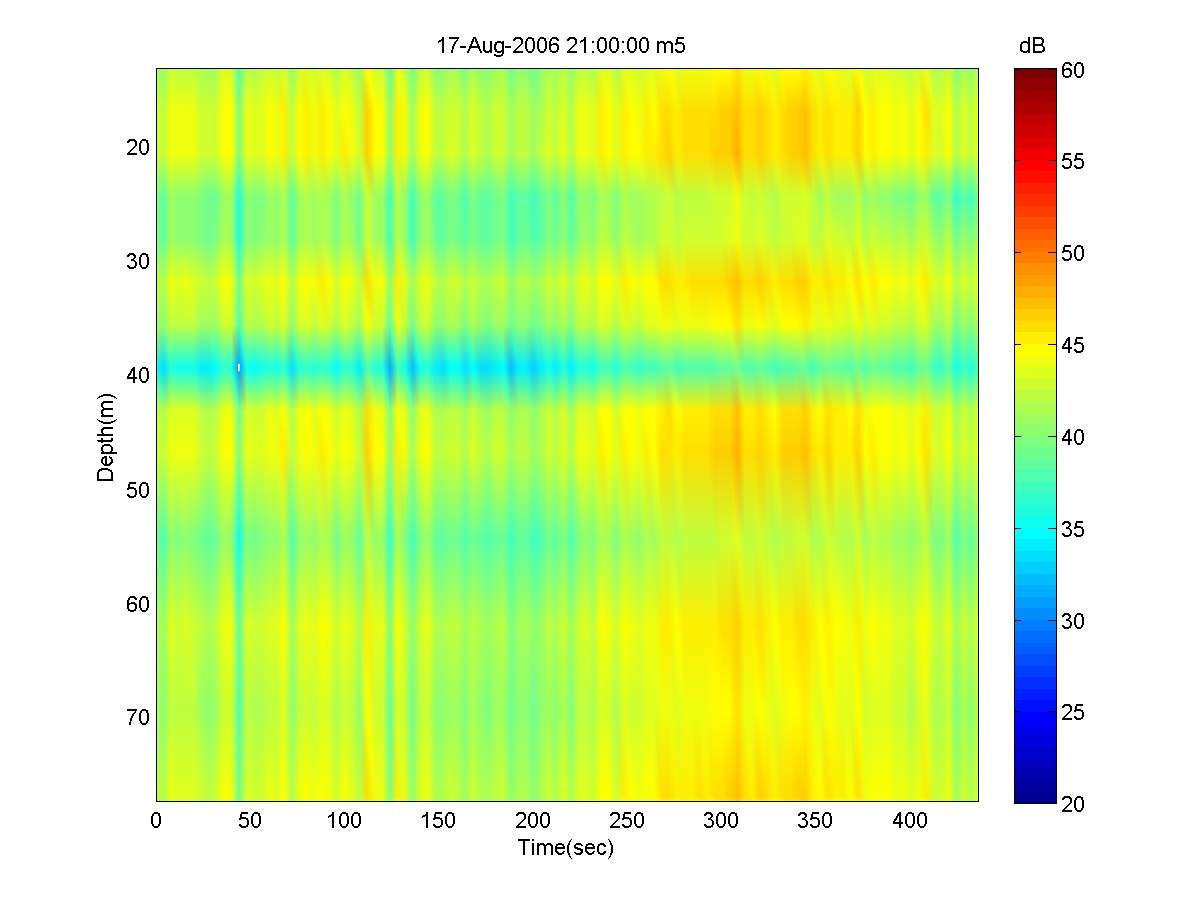
\includegraphics[width=0.3\textwidth,height=0.1\textwidth]{nrl_200608172100_m5.png}\\
  %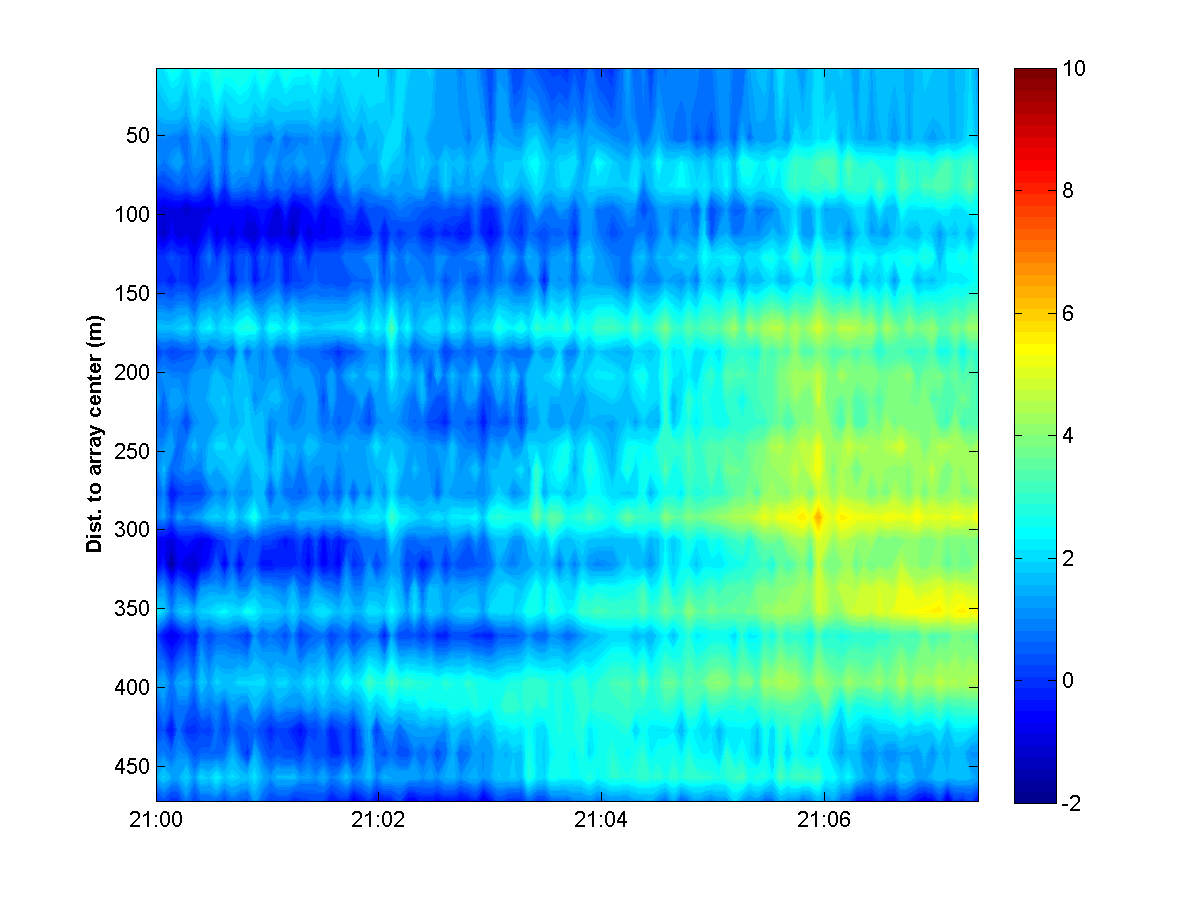
\includegraphics[width=0.3\textwidth,height=0.1\textwidth]{0817_2100_hla.png}
  %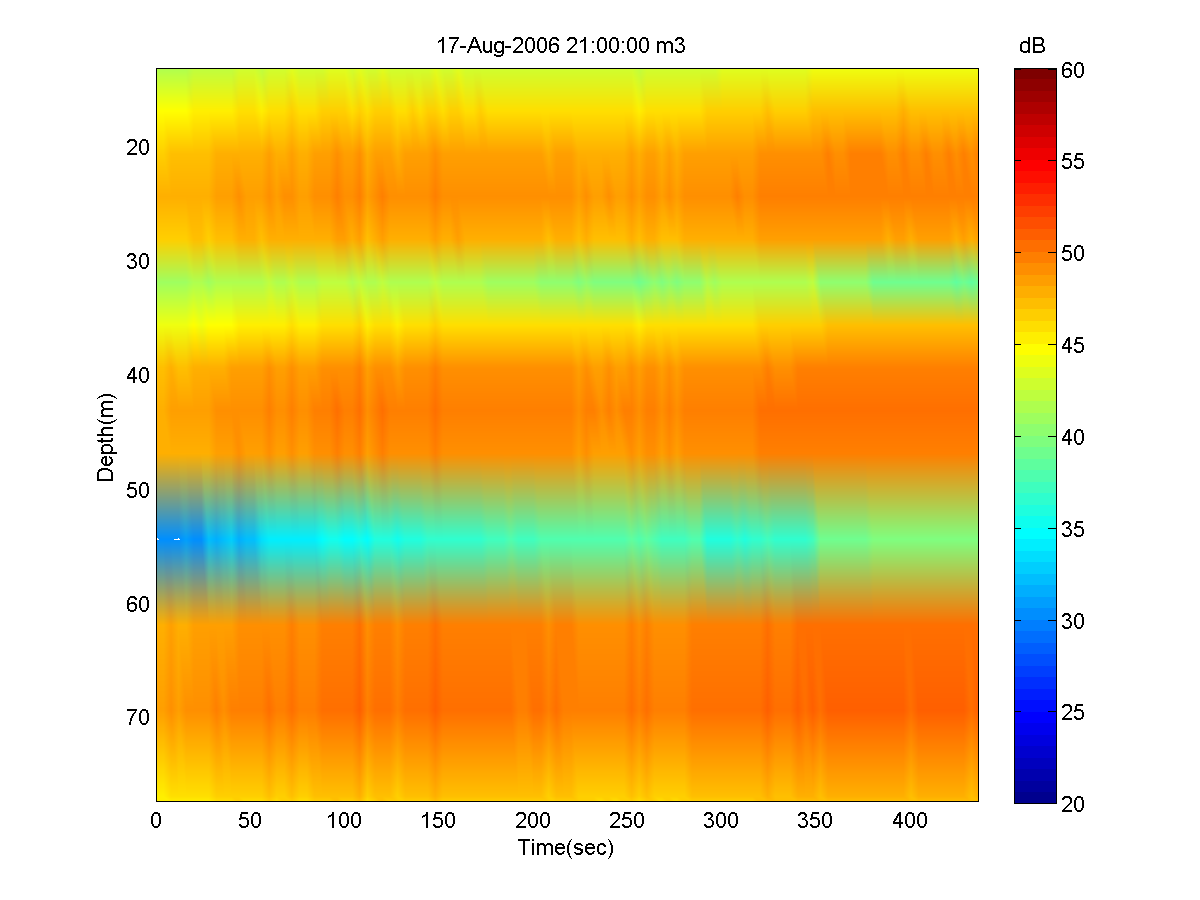
\includegraphics[width=0.3\textwidth,height=0.1\textwidth]{nrl_200608172100_m3.png}
  %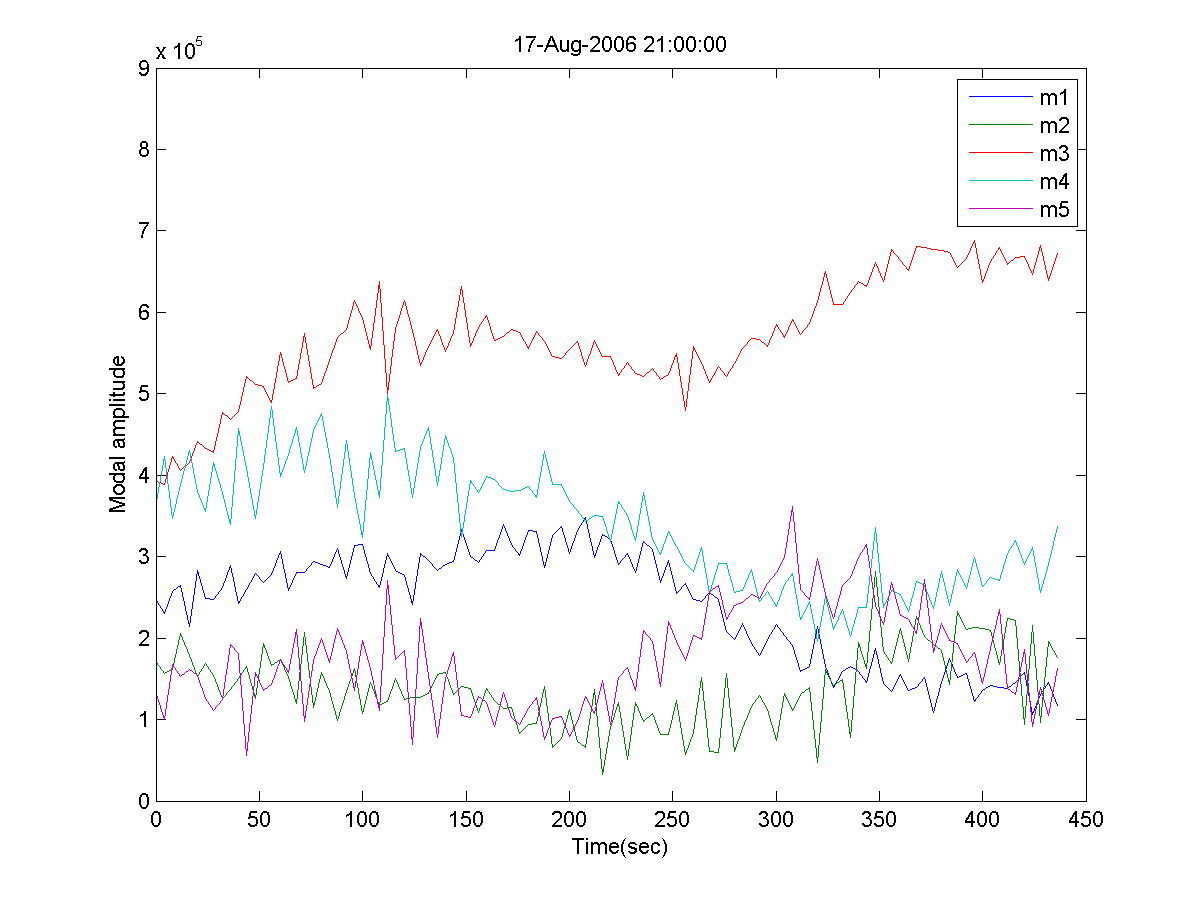
\includegraphics[width=0.3\textwidth,height=0.1\textwidth]{nrl_ma_200608172100.png}\\
  %\end{tabular}
  %\caption{Received signal on Shark array from Aug.17 21:00GMT to 21:07GMT. Left column, from top to bottom: signal on VLA, VLA signal intensity, signal on HLA; middle column: mode 1-3; right column: mode 4, 5, and modal amplitudes.}\label{fig:m2100}
%\end{figure}
\subsubsection{21:30GMT-21:37GMT}
Figure \ref{fig:r2130_r} shows the radar images taken at 21:37GMT. The interpolated temperature field is shown in Figure \ref{fig:r2130_i} (water depth = 20m). 

Radar image shows the major ISW reaches the VLA at about 21:37GMT,
but the signal received on SHARK VLA and HLA shows the effects of
ISW on the acoustic propagation starts a bit earlier at about
21:33GMT when the HLA shows the slope caused by the movement of the
ISW. A 5dB dip on the total intensity plot implies the energy could
be transferred out of the VLA plane. Mode 1 and 2 are steady and
strong when pushed to the deeper water by the downward movement of
the thermocline. On the other hand, mode 3, 4 and 5 show strong
(~8dB) and fast(period = 50sec) oscillation starting about 21:33GMT,
confirming the effects of ISW on acoustic propagation.



%\begin{figure}[H]
%  \centering
%  \begin{tabular}{l}
%  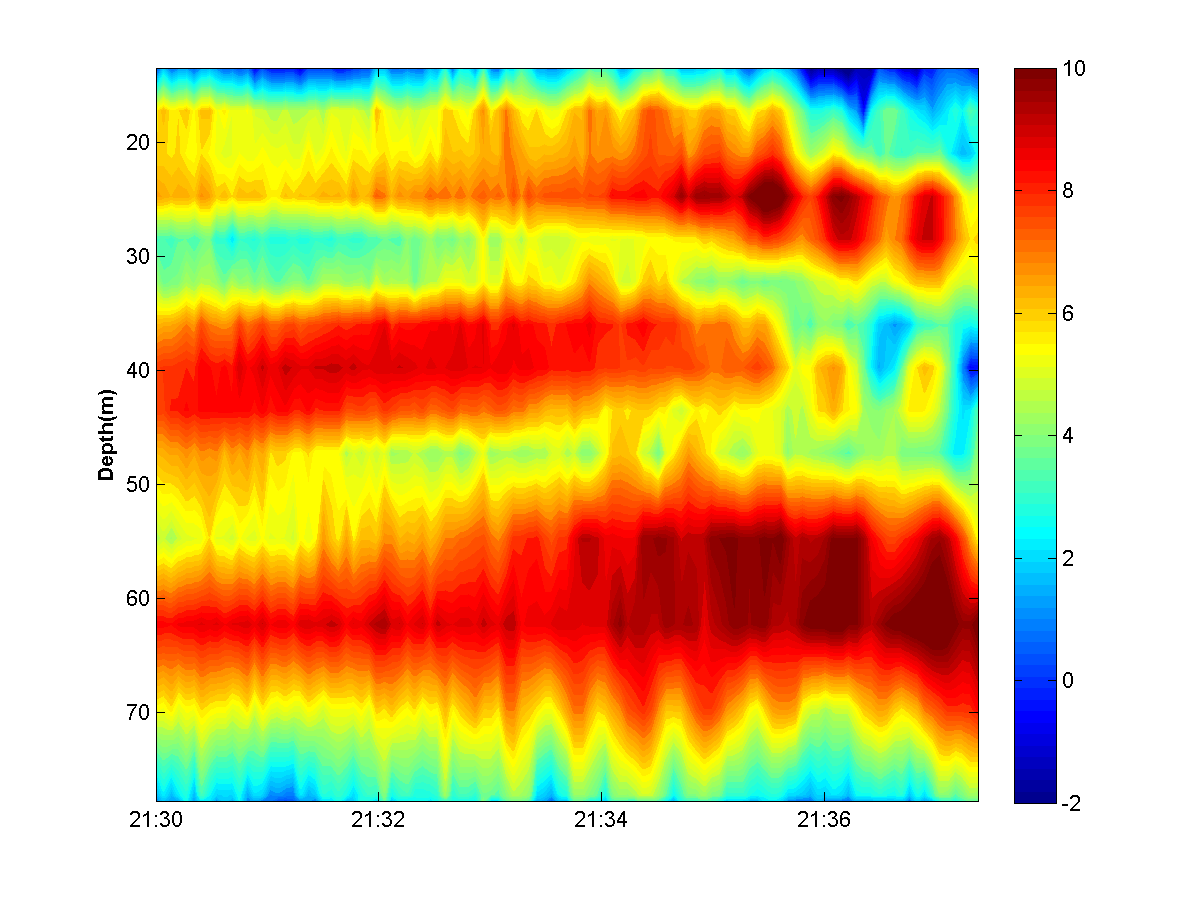
\includegraphics[width=0.5\textwidth,height=0.2\textwidth]{0817_2130_vla.png}\\
%  \ 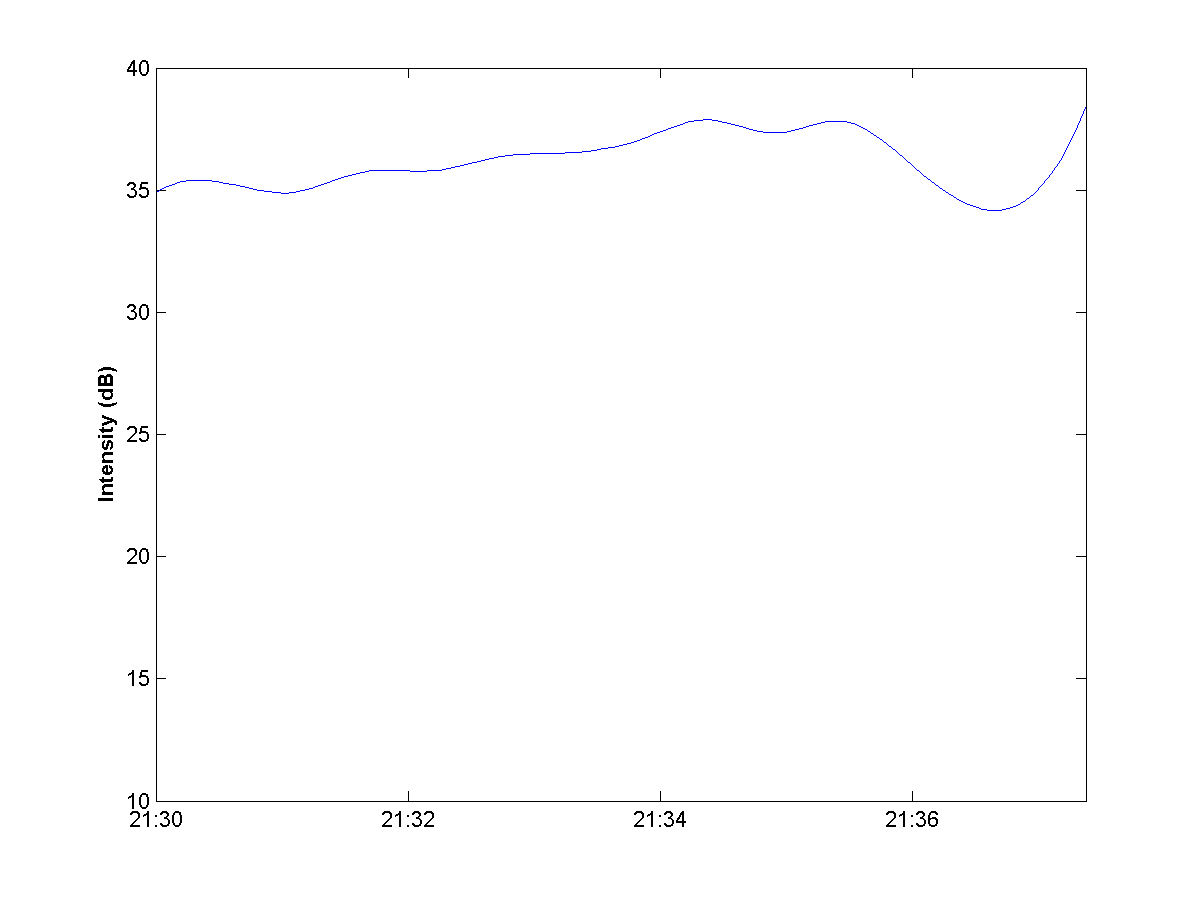
\includegraphics[width=0.44\textwidth,height=0.2\textwidth]{0817_2130_eng.png}\\
%  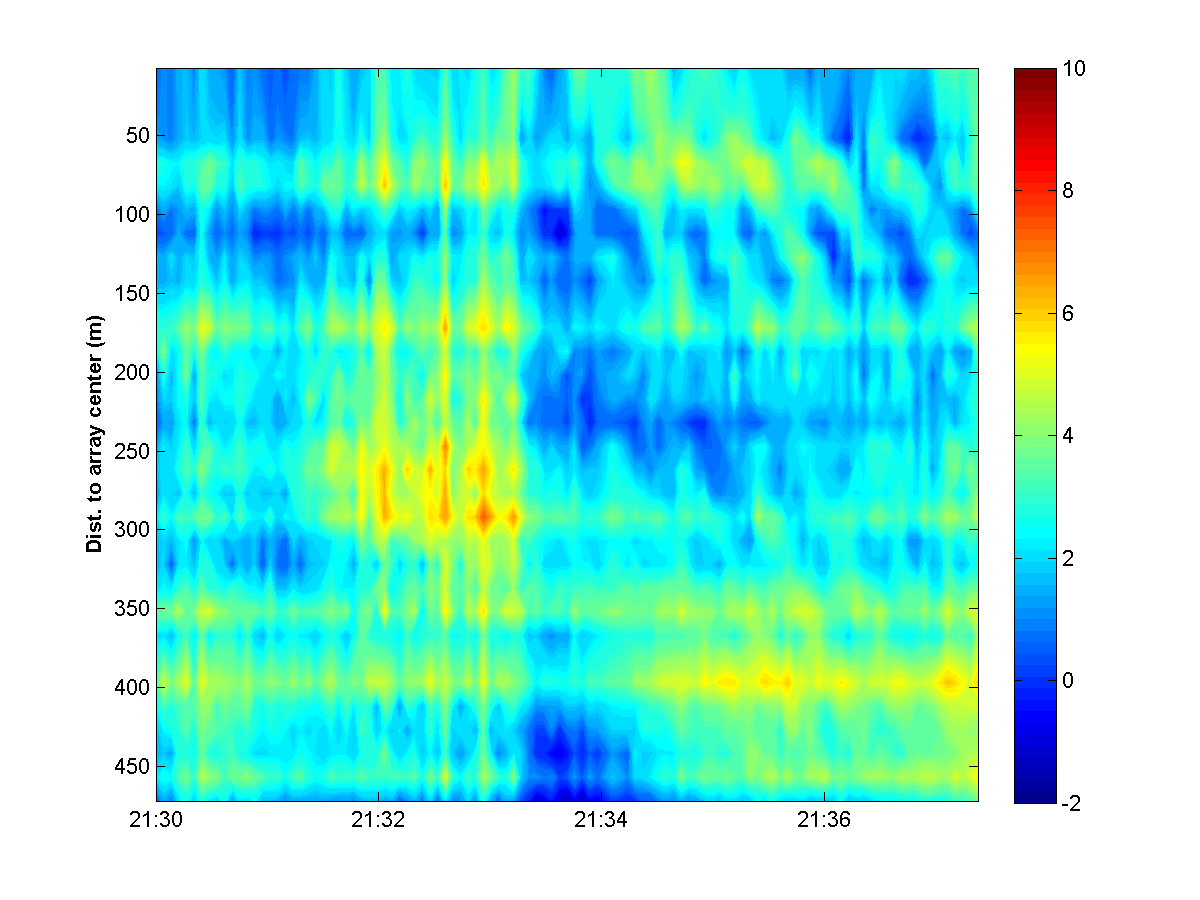
\includegraphics[width=0.5\textwidth,height=0.2\textwidth]{0817_2130_hla.png}\\
%  \end{tabular}
%  \caption{Received signal on Shark VLA (top), HLA (bottom) and signal intensity (middle) from Aug.17 21:30GMT to 21:37GMT }\label{fig:a2130}
%\end{figure}
%
%\begin{figure}[H]
%  \centering
%  \begin{tabular}{cc}
%  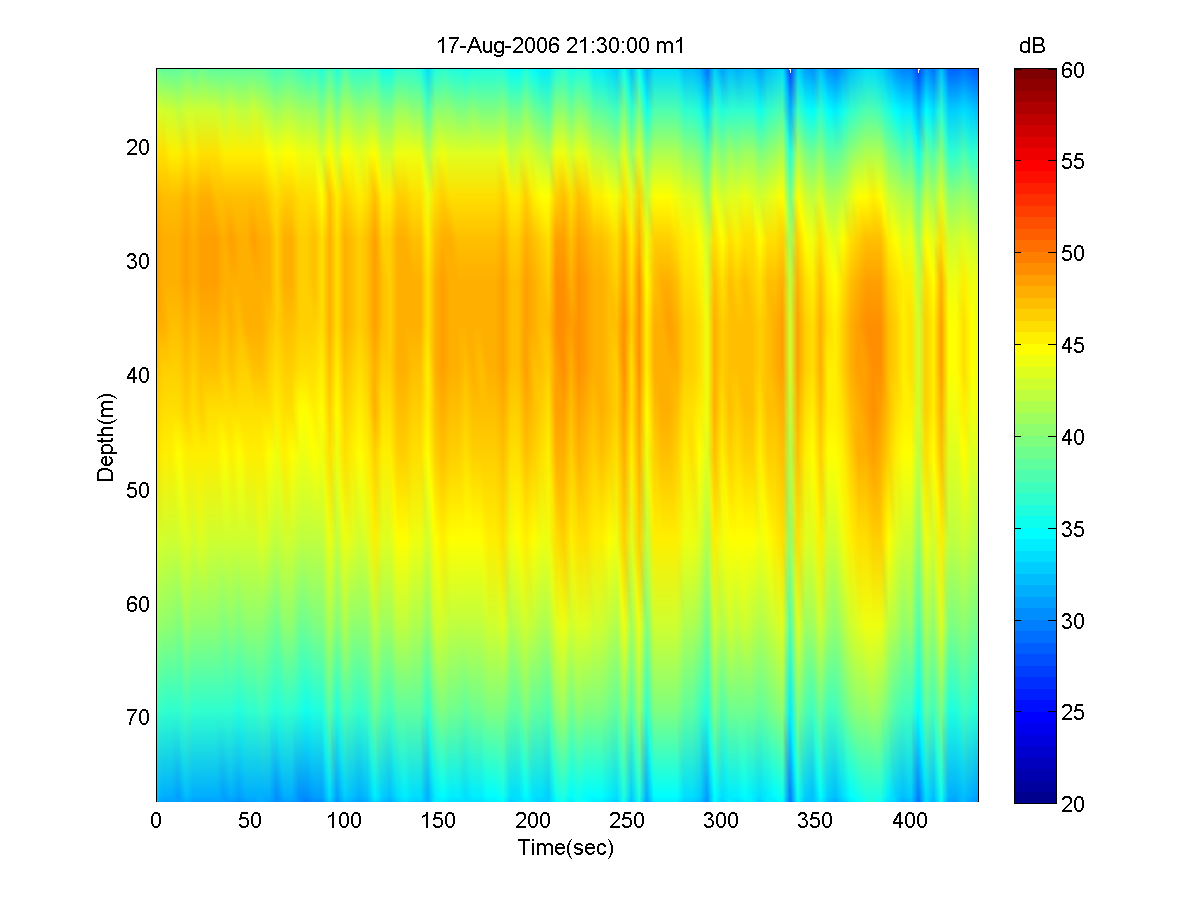
\includegraphics[width=0.5\textwidth,height=0.2\textwidth]{nrl_200608172130_m1.png}
%  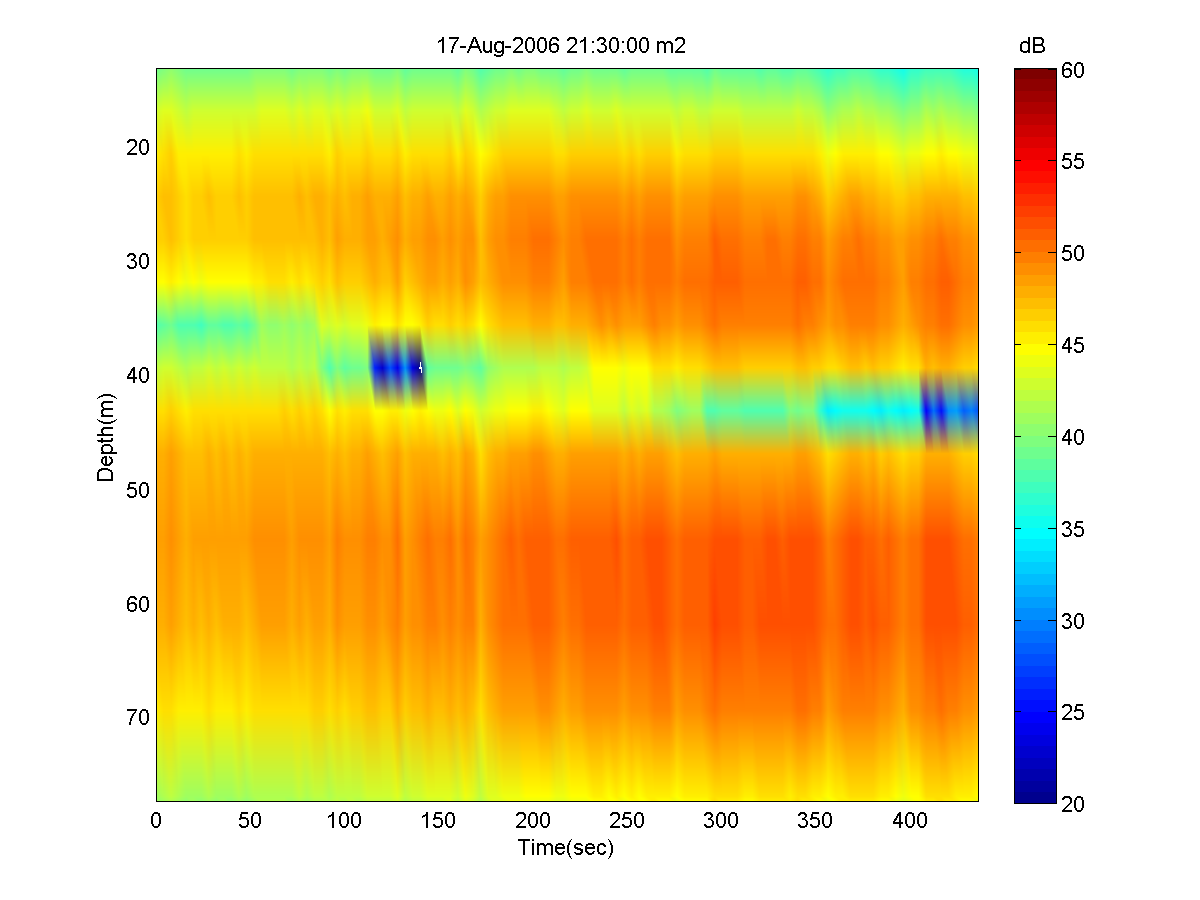
\includegraphics[width=0.5\textwidth,height=0.2\textwidth]{nrl_200608172130_m2.png}\\
%  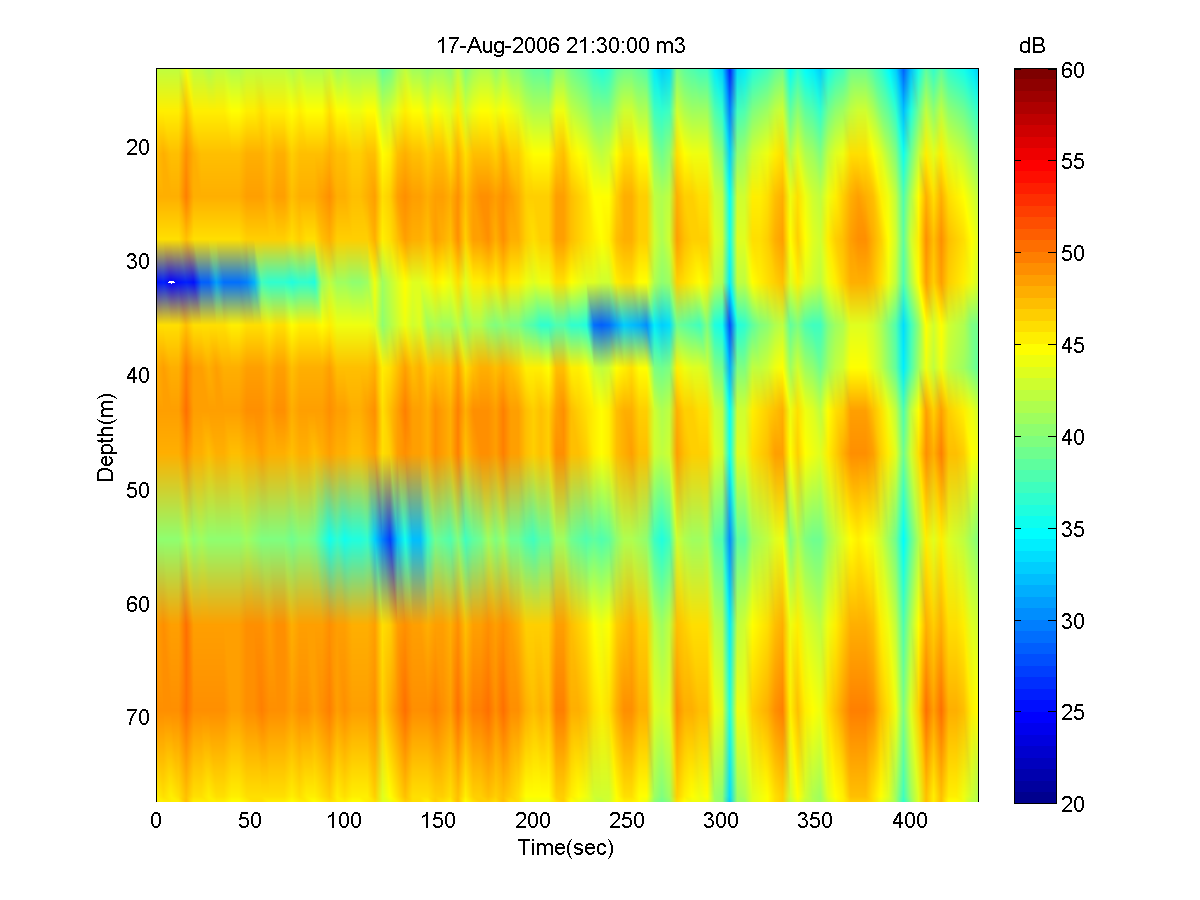
\includegraphics[width=0.5\textwidth,height=0.2\textwidth]{nrl_200608172130_m3.png}
%  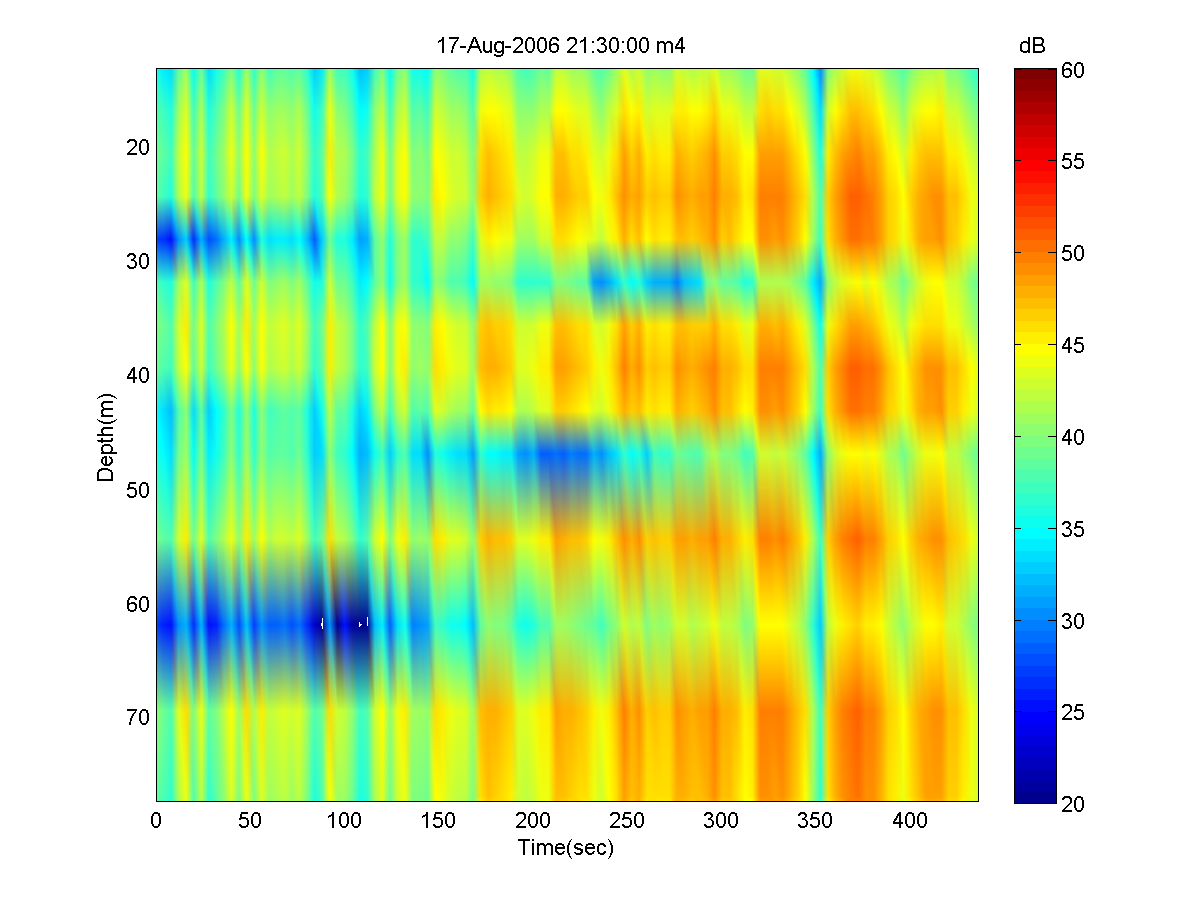
\includegraphics[width=0.5\textwidth,height=0.2\textwidth]{nrl_200608172130_m4.png}\\
%  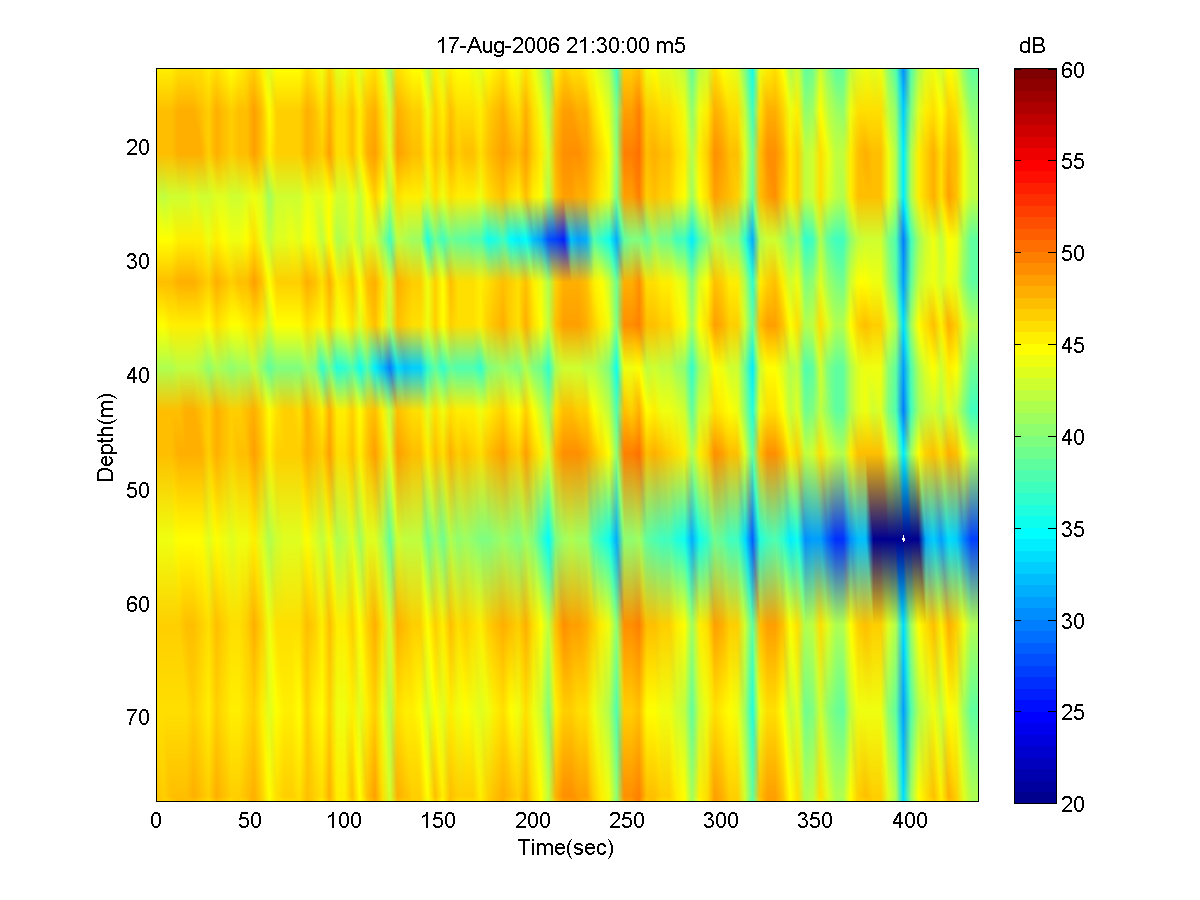
\includegraphics[width=0.5\textwidth,height=0.2\textwidth]{nrl_200608172130_m5.png}
%  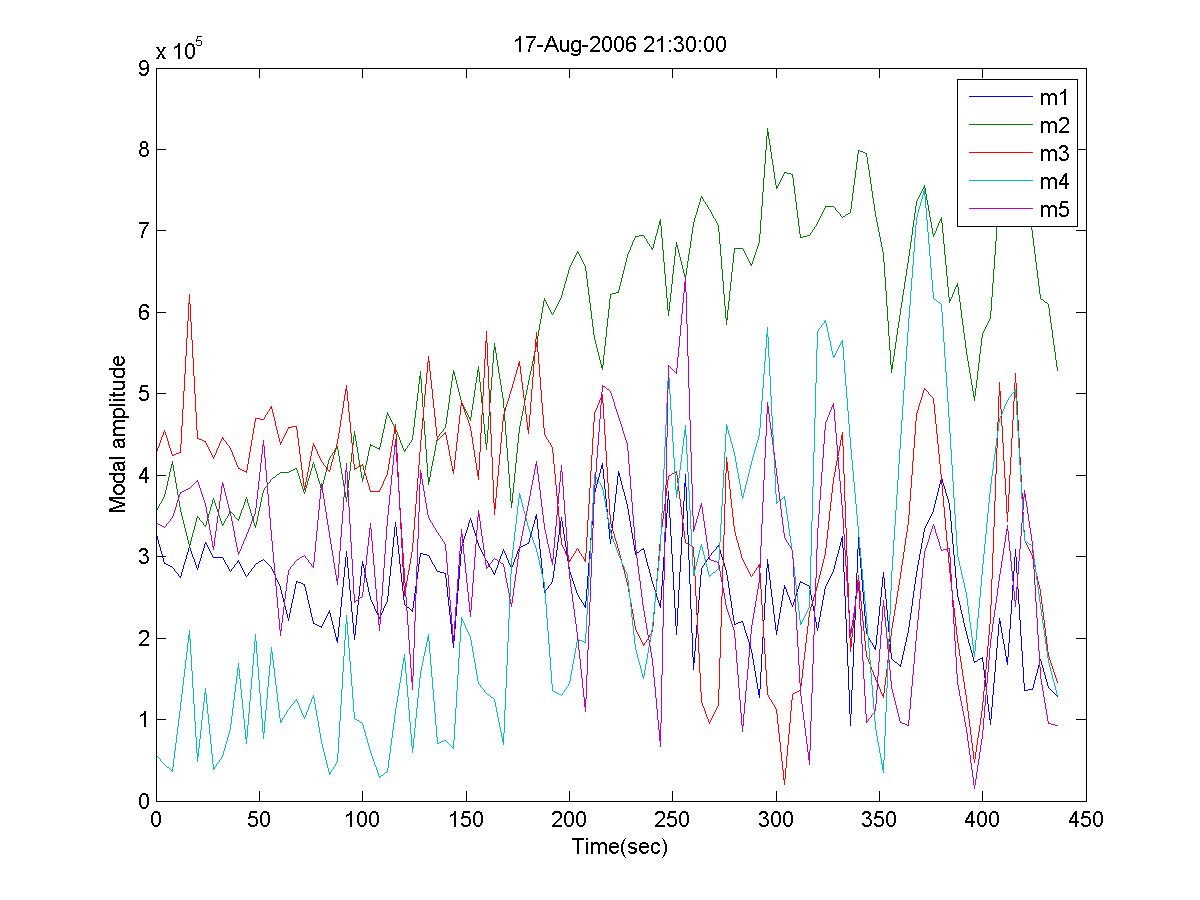
\includegraphics[width=0.5\textwidth,height=0.2\textwidth]{nrl_ma_200608172130.png}\\
%  \end{tabular}
%  \caption{Modal decomposition and amplitude of the signal received on Shark VLA from Aug.17 21:30GMT to 21:37GMT }\label{fig:m2130}
%\end{figure}

%\begin{figure}
 % \centering
  %\begin{tabular}{lrr}
  %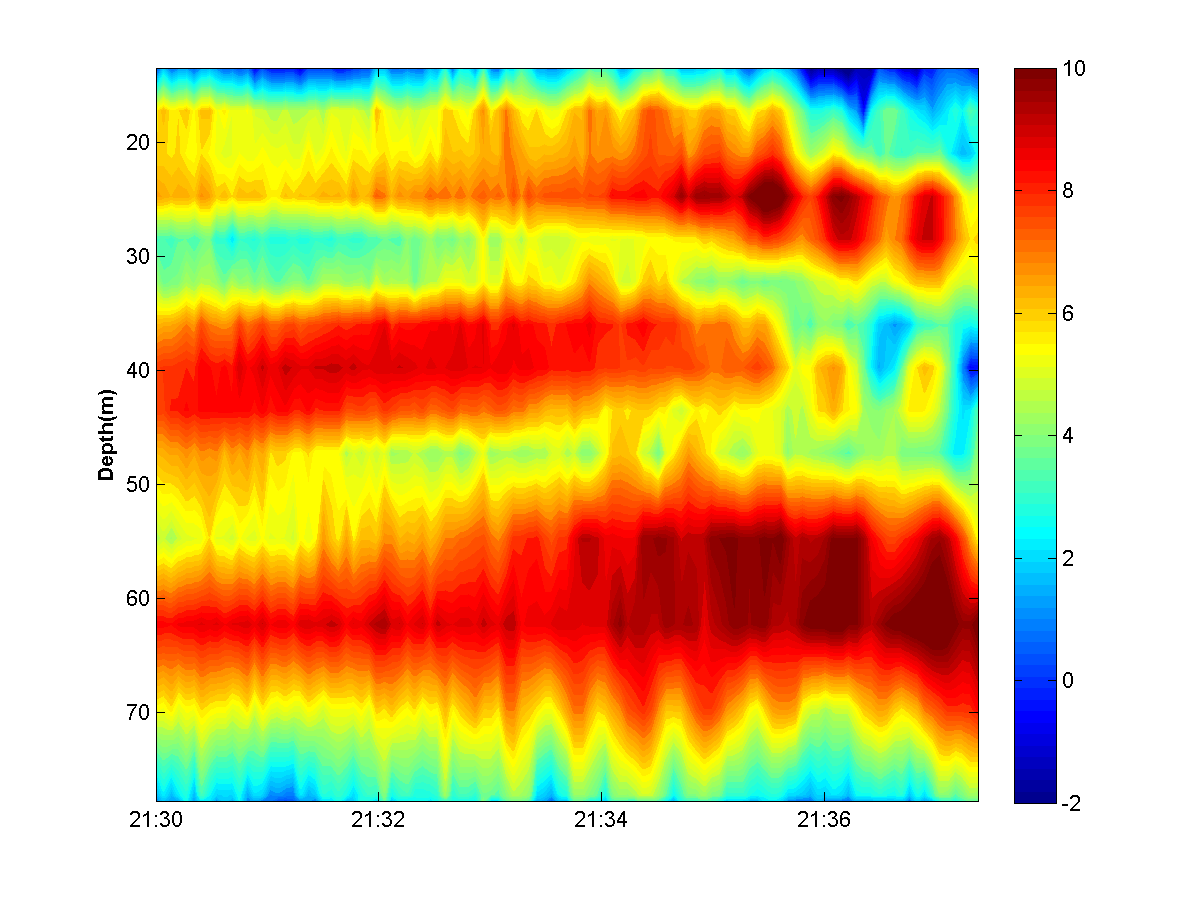
\includegraphics[width=0.3\textwidth,height=0.1\textwidth]{0817_2130_vla.png}
  %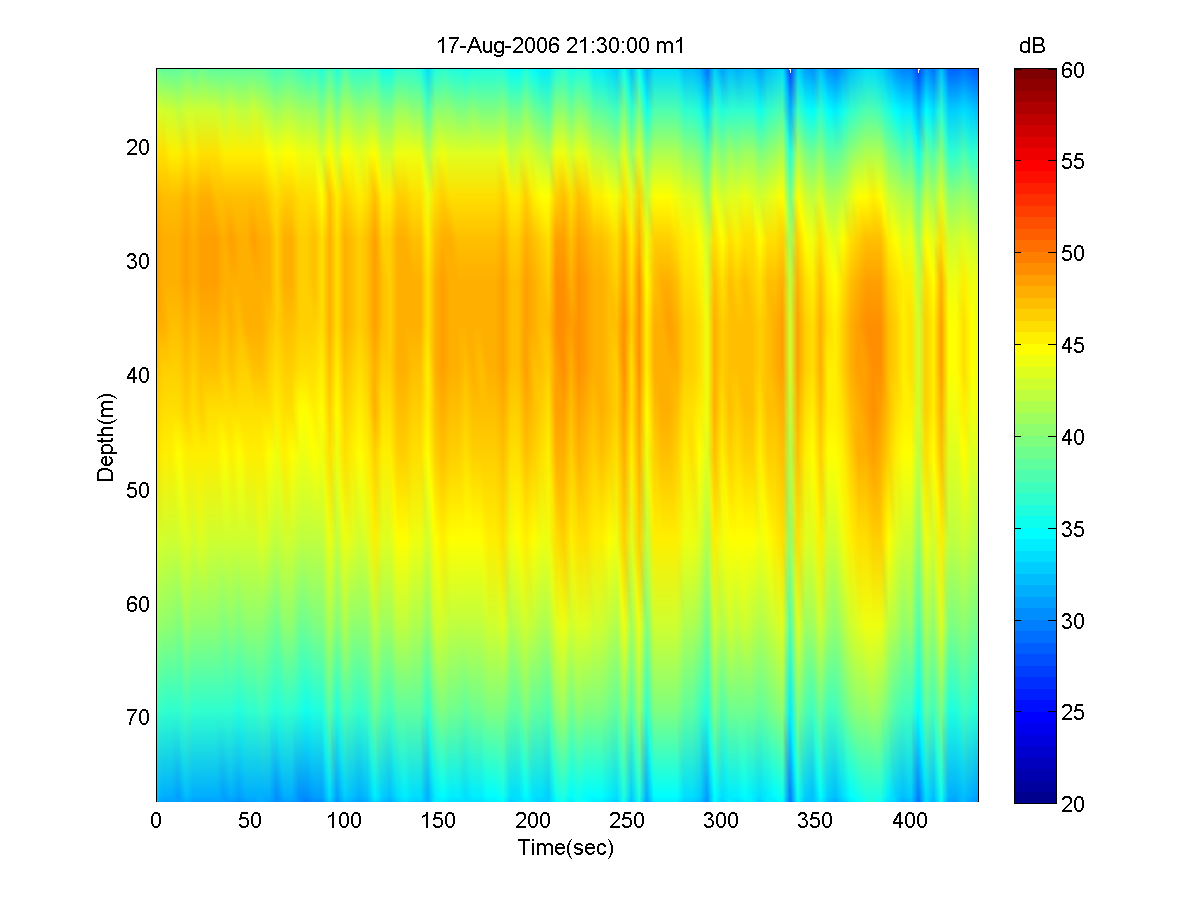
\includegraphics[width=0.3\textwidth,height=0.1\textwidth]{nrl_200608172130_m1.png}
  %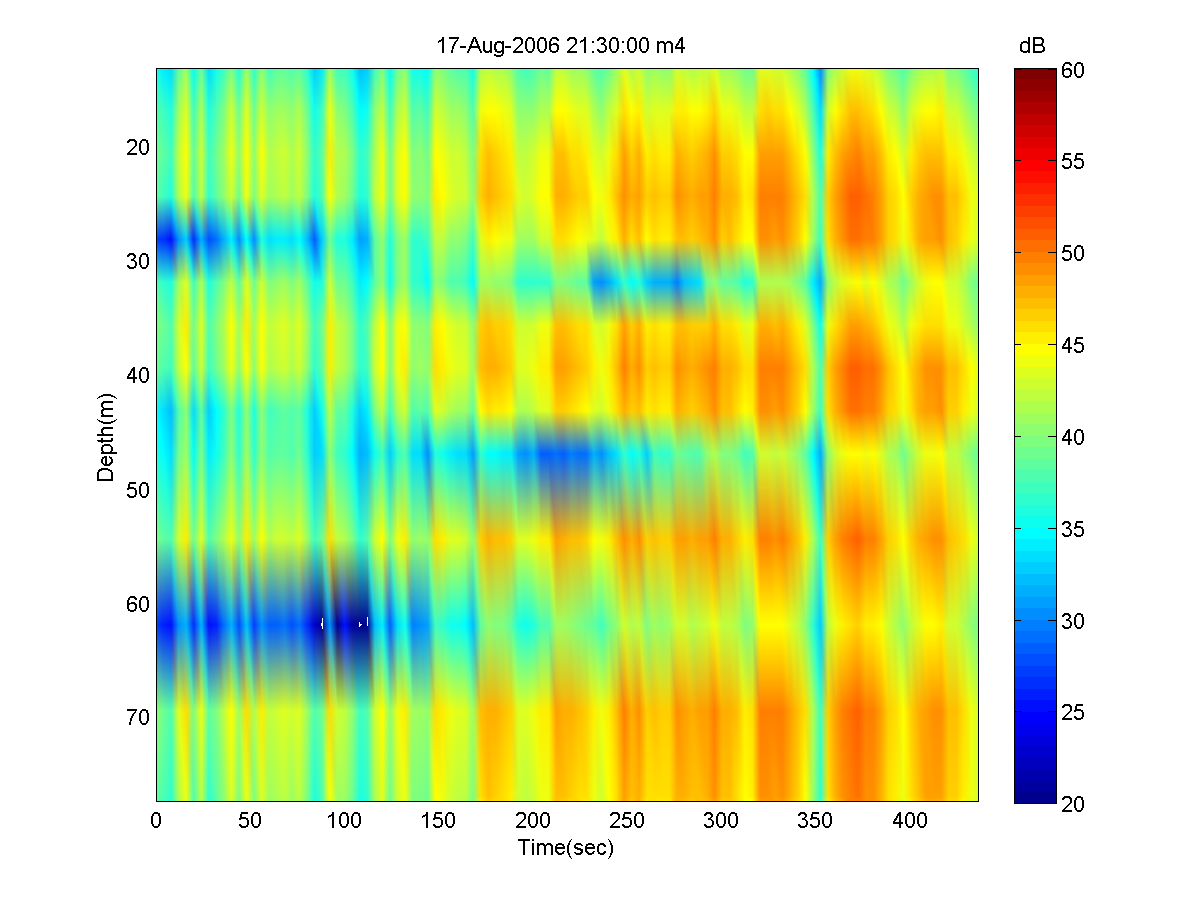
\includegraphics[width=0.3\textwidth,height=0.1\textwidth]{nrl_200608172130_m4.png}\\
  %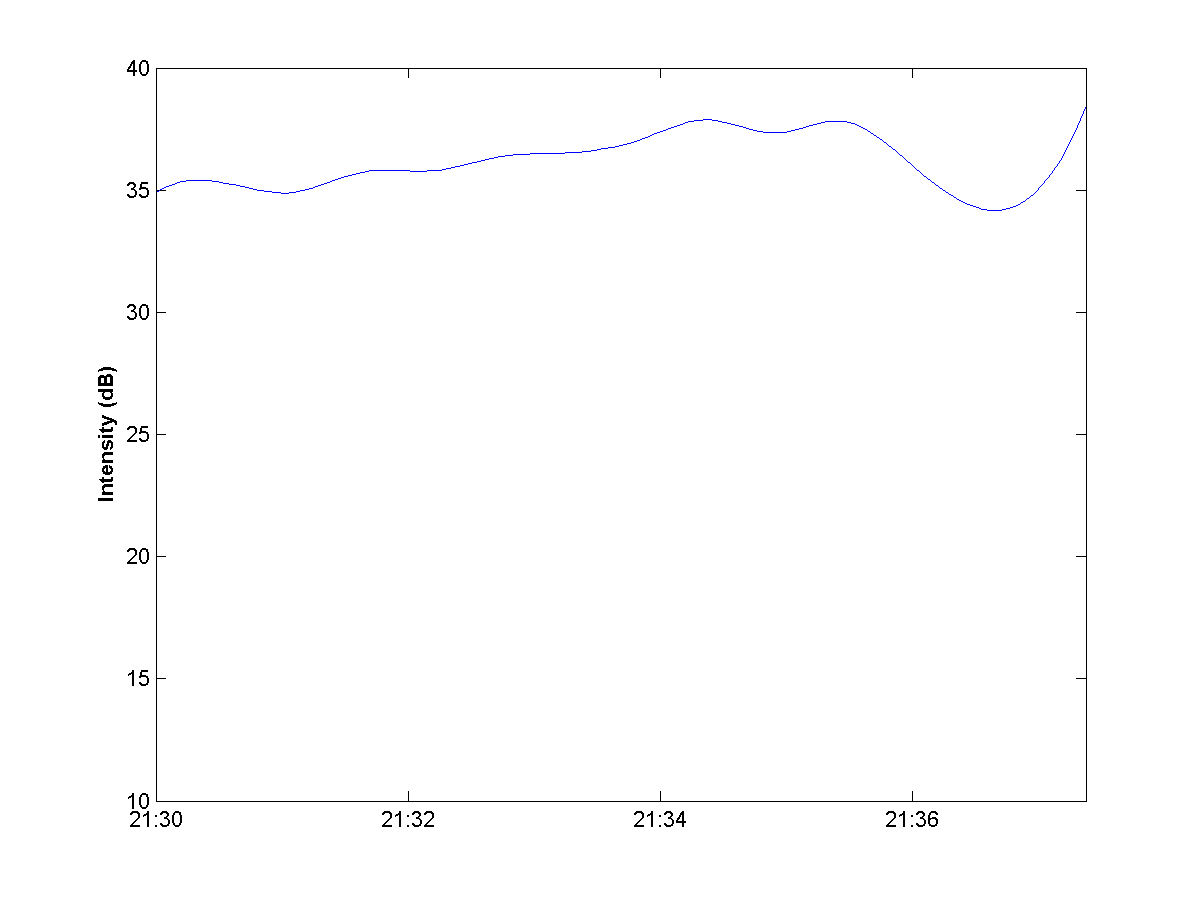
\includegraphics[width=0.3\textwidth,height=0.1\textwidth]{0817_2130_eng.png}
  %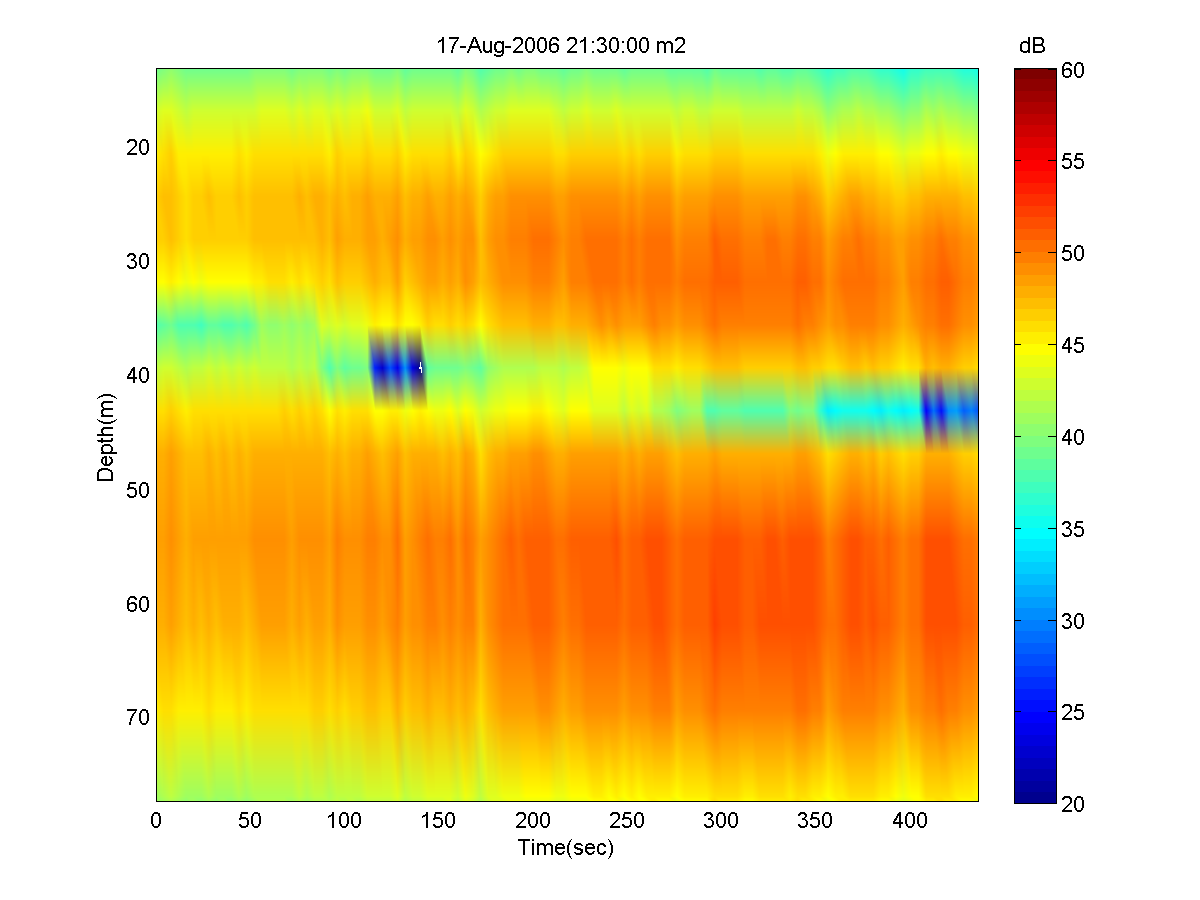
\includegraphics[width=0.3\textwidth,height=0.1\textwidth]{nrl_200608172130_m2.png}
  %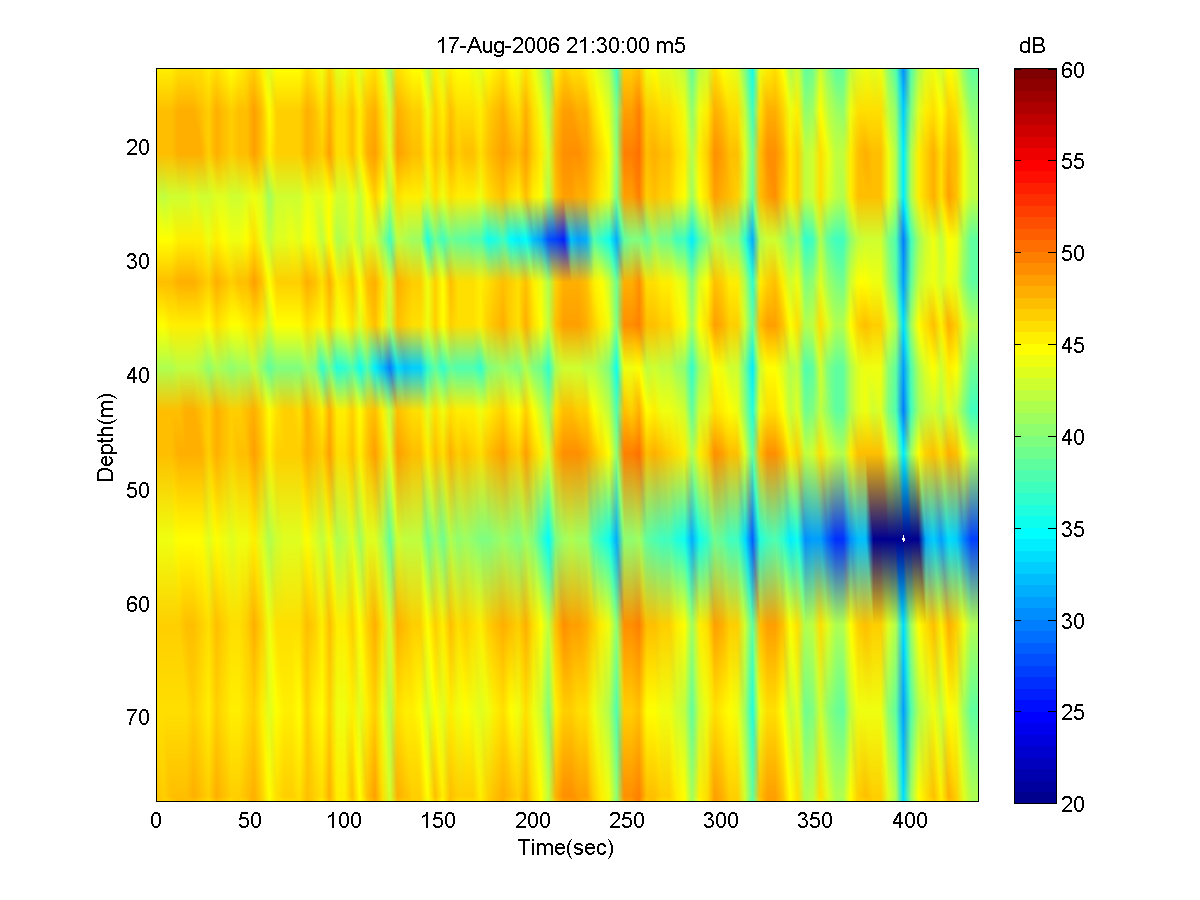
\includegraphics[width=0.3\textwidth,height=0.1\textwidth]{nrl_200608172130_m5.png}\\
  %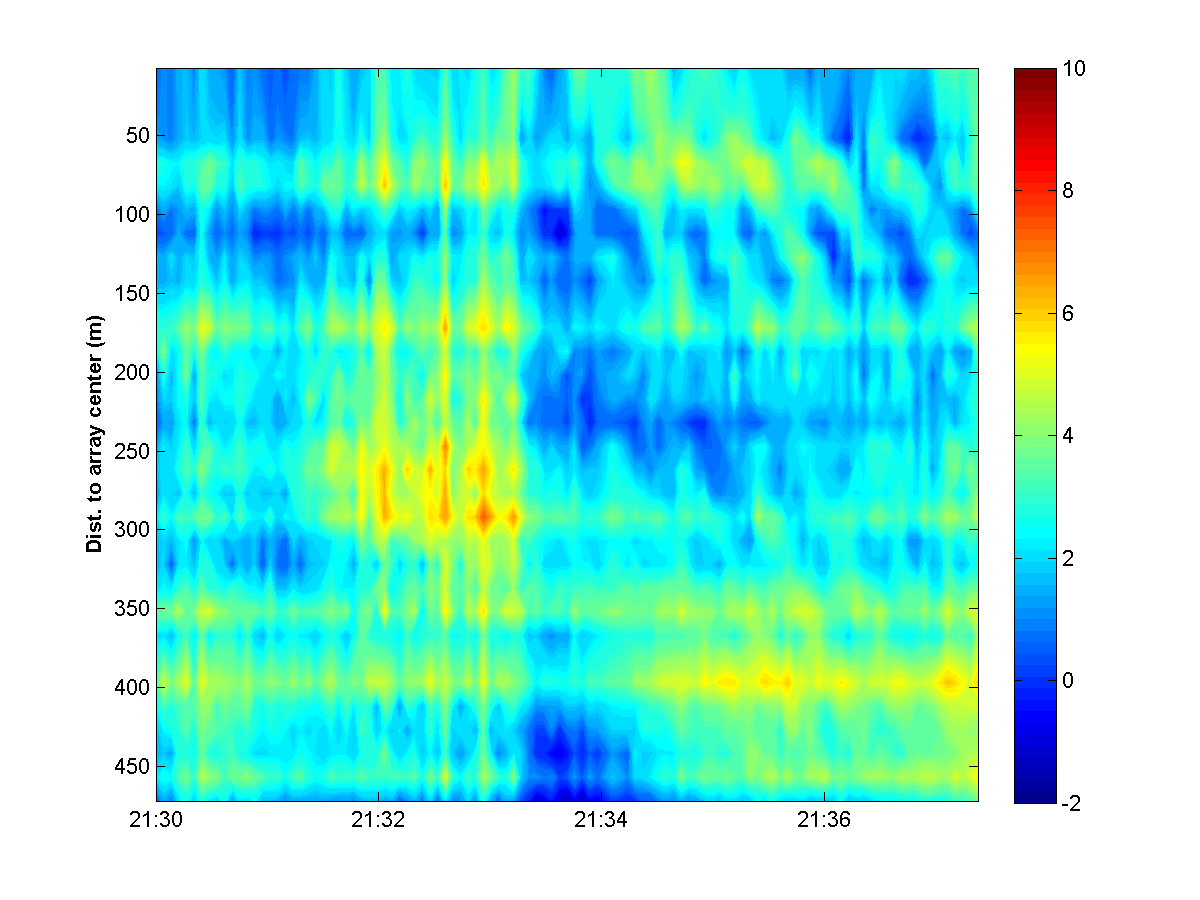
\includegraphics[width=0.3\textwidth,height=0.1\textwidth]{0817_2130_hla.png}
  %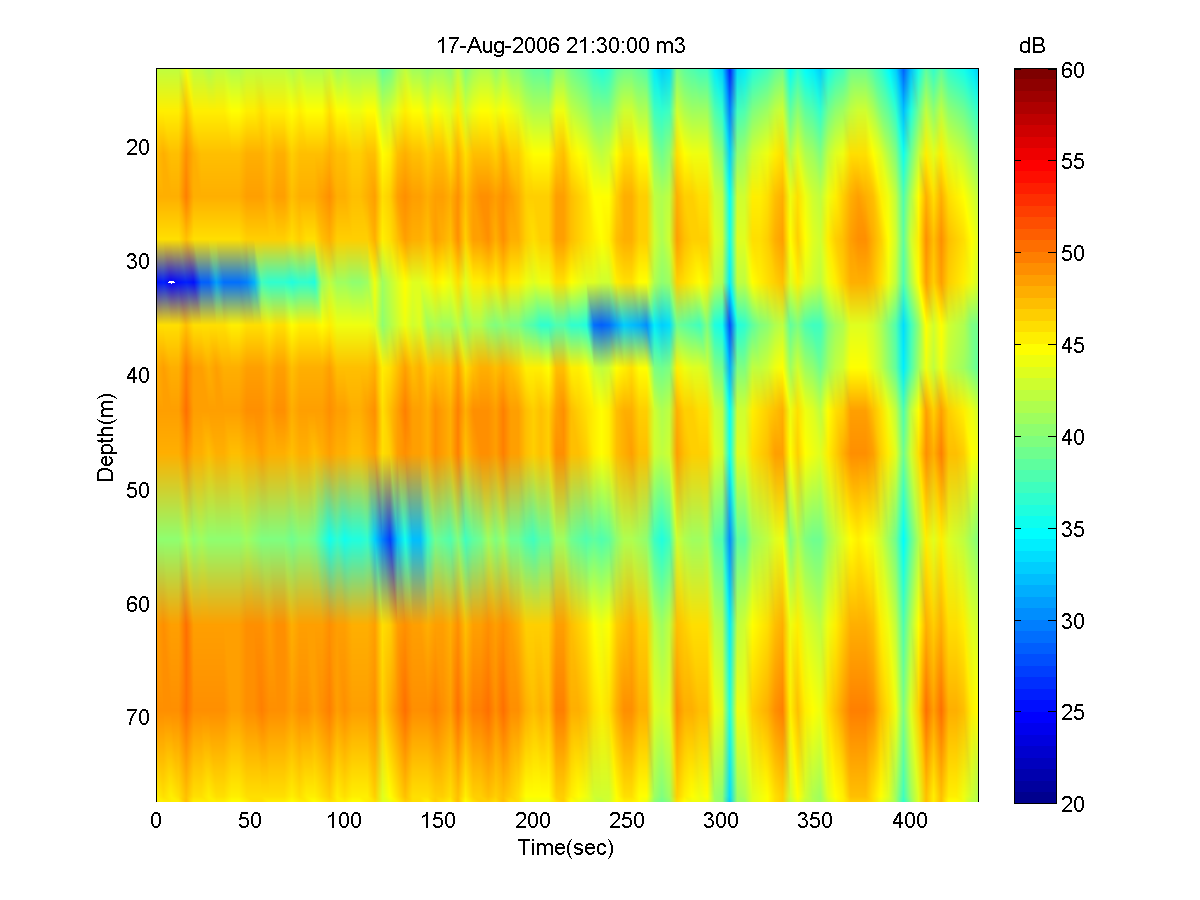
\includegraphics[width=0.3\textwidth,height=0.1\textwidth]{nrl_200608172130_m3.png}
  %\includegraphics[width=0.3\textwidth,height=0.1\textwidth]{nrl_ma_200608172130.png}\\
  %\end{tabular}
  %\caption{Received signal on Shark array from Aug.17 21:30GMT to 21:37GMT. Left column, from top to bottom: signal on VLA, VLA signal intensity, signal on HLA; middle column: mode 1-3; right column: mode 4, 5, and modal amplitudes.}\label{fig:m2130}
%\end{figure}
\subsubsection{22:00GMT-22:07GMT}
ISW occupies the most of the acoustic path. Slopes on the HLA show
the strong effects of ISW on the acoustic propagation. On the VLA,
the focusing induces the intensity fluctuation of 15dB. Modal
decomposition shows mode 1 is the dominant play of the focusing with
a sudden increase in amplitude.
%\begin{figure}[H]
 % \centering
  %\includegraphics[width=0.5\textwidth]{radar2200.png}
  %\caption{Radar image of ISW at 21:30GMT}\label{fig:r2200}
%\end{figure}
%\begin{figure}
 % \centering
  %\begin{tabular}{lrr}
  %\includegraphics[width=0.3\textwidth,height=0.1\textwidth]{0817_2200_vla.png}
  %\includegraphics[width=0.3\textwidth,height=0.1\textwidth]{nrl_200608172200_m1.png}
  %\includegraphics[width=0.3\textwidth,height=0.1\textwidth]{nrl_200608172200_m4.png}\\
  %\includegraphics[width=0.3\textwidth,height=0.1\textwidth]{0817_2200_eng.png}
  %\includegraphics[width=0.3\textwidth,height=0.1\textwidth]{nrl_200608172200_m2.png}
  %\includegraphics[width=0.3\textwidth,height=0.1\textwidth]{nrl_200608172200_m5.png}\\
  %\includegraphics[width=0.3\textwidth,height=0.1\textwidth]{0817_2200_hla.png}
  %\includegraphics[width=0.3\textwidth,height=0.1\textwidth]{nrl_200608172200_m3.png}
  %\includegraphics[width=0.3\textwidth,height=0.1\textwidth]{nrl_ma_200608172200.png}\\
  %\end{tabular}
  %\caption{Received signal on Shark array from Aug.17 20:30GMT to 20:37GMT. Left column, from top to bottom: signal on VLA, VLA signal intensity, signal on HLA; middle column: mode 1-3; right column: mode 4, 5, and modal amplitudes.}\label{fig:m2200}
%\end{figure}
\subsubsection{22:30GMT-22:37GMT}
The acoustic path is at the middle of the ISW package, where the
wavelength is shorter than the leading fronts. Two focusing events
are observed with 15dB variations on total intensity. Mode 1 and 2
show more fluctuation than mode 3, 4 and 5. On HLA, regular slopes
are shown, sometimes not consistent with the signals on VLA.
%\begin{figure}[H]
 % \centering
  %\includegraphics[width=0.5\textwidth]{radar2230.png}
  %\caption{Radar image of ISW at 21:30GMT}\label{fig:r2230}
%\end{figure}
%\begin{figure}
  %\centering
  %\begin{tabular}{lrr}
  %\includegraphics[width=0.3\textwidth,height=0.1\textwidth]{0817_2230_vla.png}
  %\includegraphics[width=0.3\textwidth,height=0.1\textwidth]{nrl_200608172230_m1.png}
  %\includegraphics[width=0.3\textwidth,height=0.1\textwidth]{nrl_200608172230_m4.png}\\
  %\includegraphics[width=0.3\textwidth,height=0.1\textwidth]{0817_2230_eng.png}
  %\includegraphics[width=0.3\textwidth,height=0.1\textwidth]{nrl_200608172230_m2.png}
  %\includegraphics[width=0.3\textwidth,height=0.1\textwidth]{nrl_200608172230_m5.png}\\
  %\includegraphics[width=0.3\textwidth,height=0.1\textwidth]{0817_2230_hla.png}
  %\includegraphics[width=0.3\textwidth,height=0.1\textwidth]{nrl_200608172230_m3.png}
  %\includegraphics[width=0.3\textwidth,height=0.1\textwidth]{nrl_ma_200608172230.png}\\
  %\end{tabular}
  %\caption{Received signal on Shark array from Aug.17 22:30GMT to 22:37GMT. Left column, from top to bottom: signal on VLA, VLA signal intensity, signal on HLA; middle column: mode 1-3; right column: mode 4, 5, and modal amplitudes.}\label{fig:m2230}
%\end{figure}
\subsubsection{23:00GMT-23:07GMT}
The acoustic path now is at the coverage of R/V Sharp's radar, and
escapes from R/V Oceanouse's radar. From the temperature plot, the
acoustic path is still affected by the ISW package. Tow focusing
events are shown with about 15dB fluctuation.
%\begin{figure}[H]
 % \centering
%  \includegraphics[width=0.5\textwidth]{radar2300.png}
 % \caption{Radar image of ISW at 21:30GMT}\label{fig:r2300}
%\end{figure}
%\begin{figure}
 % \centering
  %\begin{tabular}{lrr}
  %\includegraphics[width=0.3\textwidth,height=0.1\textwidth]{0817_2300_vla.png}
  %\includegraphics[width=0.3\textwidth,height=0.1\textwidth]{nrl_200608172300_m1.png}
  %\includegraphics[width=0.3\textwidth,height=0.1\textwidth]{nrl_200608172300_m4.png}\\
  %\includegraphics[width=0.3\textwidth,height=0.1\textwidth]{0817_2300_eng.png}
  %\includegraphics[width=0.3\textwidth,height=0.1\textwidth]{nrl_200608172300_m2.png}
  %\includegraphics[width=0.3\textwidth,height=0.1\textwidth]{nrl_200608172300_m5.png}\\
  %\includegraphics[width=0.3\textwidth,height=0.1\textwidth]{0817_2300_hla.png}
  %\includegraphics[width=0.3\textwidth,height=0.1\textwidth]{nrl_200608172300_m3.png}
  %\includegraphics[width=0.3\textwidth,height=0.1\textwidth]{nrl_ma_200608172300.png}\\
  %\end{tabular}
  %\caption{Received signal on Shark array from Aug.17 23:00GMT to 23:07GMT. Left column, from top to bottom: signal on VLA, VLA signal intensity, signal on HLA; middle column: mode 1-3; right column: mode 4, 5, and modal amplitudes.}\label{fig:m2300}
%\end{figure}
\subsubsection{23:30GMT-23:37GMT}
No radar image, but the temperature plots shows the acoustic path is
still under the influence of ISW. Tow focusing events are recorded
on HLA with fluctuation about 15dB.
%\begin{figure}[H]
 % \centering
 % \includegraphics[width=0.5\textwidth]{radar2330.png}
  %\caption{Radar image of ISW at 21:30GMT}\label{fig:r2330}
%\end{figure}
%\begin{figure}
  %\centering
  %\begin{tabular}{lrr}
  %\includegraphics[width=0.3\textwidth,height=0.1\textwidth]{0817_2330_vla.png}
  %\includegraphics[width=0.3\textwidth,height=0.1\textwidth]{nrl_200608172330_m1.png}
  %\includegraphics[width=0.3\textwidth,height=0.1\textwidth]{nrl_200608172330_m4.png}\\
  %\includegraphics[width=0.3\textwidth,height=0.1\textwidth]{0817_2330_eng.png}
  %\includegraphics[width=0.3\textwidth,height=0.1\textwidth]{nrl_200608172330_m2.png}
  %\includegraphics[width=0.3\textwidth,height=0.1\textwidth]{nrl_200608172330_m5.png}\\
  %\includegraphics[width=0.3\textwidth,height=0.1\textwidth]{0817_2330_hla.png}
  %\includegraphics[width=0.3\textwidth,height=0.1\textwidth]{nrl_200608172330_m3.png}
  %\includegraphics[width=0.3\textwidth,height=0.1\textwidth]{nrl_ma_200608172330.png}\\
  %\end{tabular}
  %\caption{Received signal on Shark array from Aug.17 23:30GMT to 23:37GMT. Left column, from top to bottom: signal on VLA, VLA signal intensity, signal on HLA; middle column: mode 1-3; right column: mode 4, 5, and modal amplitudes.}\label{fig:m2330}
%\end{figure}


%%------------------------------------------------%%
